\documentclass[a4paper,11pt]{article}

\usepackage{ucs}
\usepackage[utf8x]{inputenc}
\usepackage[english]{babel}
\usepackage{eurosym}
\usepackage{lastpage}
\usepackage{xspace}
\usepackage[margin=15mm,includehead,includefoot]{geometry}
\usepackage{fancyhdr}
\usepackage{booktabs}
\usepackage{graphicx}
\usepackage{multirow}
\usepackage{array}
\usepackage{xcolor}
\usepackage{pgfgantt}
\usepackage{titlesec}
\usepackage{csquotes}
% \usepackage[style=verbose-ibid,backend=bibtex]{biblatex}
% \bibliography{library}
\usepackage{hyperref}
\usepackage{enumitem}
\usepackage{amsfonts}
\usepackage{amsmath}
\usepackage{amssymb}
\usepackage{wrapfig}
\usepackage{lipsum}
\usepackage{xstring}

/home/emilien/tex/tex_commons/newcommands.tex
{\newcommand{\cmsSymbolFace}{\text}
\newcommand{\PT}{\ensuremath{p_{\text{T}}}\xspace}
\newcommand{\pt}{\ensuremath{p_{\text{T}}}\xspace}
\newcommand{\cm}{\ensuremath{\,\text{cm}}\xspace}
\newcommand{\PGm}{\ensuremath{\mu}\xspace} % muon
\newcommand{\GeVc}{\ensuremath{{\,\text{Ge\hspace{-.08em}V\hspace{-0.16em}/\hspace{-0.08em}}c}}\xspace}
\newcommand{\abs}[1]{\ensuremath{\lvert #1 \rvert}}

% frequently used expressions
\newcommand{\ee}{\ensuremath{e^+e^-}\xspace}
\newcommand{\mumu}{\ensuremath{\mu^+\mu^-}\xspace}
\newcommand{\eexp}[1]{\ensuremath{{\text e}^{#1}}\xspace}

% \newcommand{\qqbar}{\ensuremath{{\cmsSymbolFace{q}\overline{\cmsSymbolFace{q}}}}\xspace}
\newcommand{\QQbar}{\ensuremath{{\cmsSymbolFace{Q}\overline{\cmsSymbolFace{Q}}}}\xspace}
\newcommand{\Jpsi}{\ensuremath{\cmsSymbolFace{J}\hspace{-.08em}/\hspace{-.14em}\psi}\xspace}
\newcommand{\JPsi}{\ensuremath{\cmsSymbolFace{J}\hspace{-.08em}/\hspace{-.14em}\psi}\xspace}
\newcommand{\psiP}{\ensuremath{\psi\text{(2S)}}\xspace}
\newcommand{\B}{\ensuremath{\cmsSymbolFace{B}}\xspace}
\newcommand{\D}{\ensuremath{\cmsSymbolFace{D}}\xspace}
\newcommand{\K}{\ensuremath{\cmsSymbolFace{K}}\xspace}
\newcommand{\Dz}{\ensuremath{\cmsSymbolFace{D}^0}\xspace}

% \newcommand{\doubleRatio}{\ensuremath{\left.\left[N_{\psiP}/N_{\Jpsi}\right]_{\PbPb}\middle/\left[N_{\psiP}/N_{\Jpsi}\right]_{\pp}\right.\xspace}}
\newcommand{\doubleRatio}{\ensuremath{\left.(N_{\psiP}/N_{\Jpsi})_{\PbPb}/(N_{\psiP}/N_{\Jpsi})_{\pp}\right.\xspace}}

\newcommand{\PgU}{\ensuremath{\Upsilon}\xspace}
\newcommand{\PgUa}{\ensuremath{\Upsilon\text{(1S)}}\xspace}
\newcommand{\PgUb}{\ensuremath{\Upsilon\text{(2S)}}\xspace}
\newcommand{\PgUc}{\ensuremath{\Upsilon\text{(3S)}}\xspace}
\newcommand{\PgUbc}{\ensuremath{\Upsilon\text{(2S+3S)}}\xspace}
\newcommand{\PgUabc}{\ensuremath{\Upsilon\text{(1S,2S,3S)}}\xspace}
\newcommand{\PgUn}{\ensuremath{\Upsilon\text{(nS)}}\xspace}

\newcommand{\W}{\ensuremath{\cmsSymbolFace{W}}\xspace}
%\newcommand{\Z}{\ensuremath{\cmsSymbolFace{Z}}\xspace}

\newcommand{\dndy}{\ensuremath{dN/dy}\xspace}
\newcommand{\dnchdy}{\ensuremath{dN_{\text{ch}}/dy}\xspace}
\newcommand{\dndeta}{\ensuremath{dN/d\eta}\xspace}
\newcommand{\dnchdeta}{\ensuremath{dN_{\text{ch}}/d\eta}\xspace}
\newcommand{\dndpt}{\ensuremath{dN/d\pt}\xspace}
\newcommand{\dnchdpt}{\ensuremath{dN_{\text{ch}}/d\pt}\xspace}
\newcommand{\deta}{\ensuremath{\Delta\eta}\xspace}
\newcommand{\dphi}{\ensuremath{\Delta\phi}\xspace}

\newcommand {\npart}  {\ensuremath{N_{\text{part}}}\xspace}
\newcommand {\ncoll}  {\ensuremath{N_{\text{coll}}}\xspace}

% references to equations, figures or tables
\newcommand{\eq}[1]{Eq.~\eqref{#1}\xspace}
\newcommand{\fig}[1]{Fig.~\ref{#1}\xspace}
\newcommand{\tab}[1]{Table~\ref{#1}\xspace}

% collision types
\newcommand{\pp}{{\ensuremath{\text{pp}}}\xspace}
\newcommand{\ppbar}{\ensuremath{\text{p}\overline{\text{p}}}\xspace}
\newcommand{\pPb}{\ensuremath{\text{p}\text{Pb}}\xspace}
\newcommand{\ppb}{\ensuremath{\text{p}\text{Pb}}\xspace}
\newcommand{\PbPb}{\ensuremath{\text{PbPb}}\xspace}
\newcommand{\pbpb}{\ensuremath{\text{PbPb}}\xspace}
\newcommand{\AuAu}{\ensuremath{\text{AuAu}}\xspace}
\newcommand{\AAA}{\ensuremath{\text{AA}}\xspace}
\newcommand{\pA}{\ensuremath{\text{pA}}\xspace}
\newcommand{\raa}{\ensuremath{R_{\AAA}}\xspace}
\newcommand{\rpa}{\ensuremath{R_{\pA}}\xspace}
\newcommand{\taa}{\ensuremath{T_{\AAA}}\xspace}

% center of mass energy
\newcommand{\sqrts}{\ensuremath{\sqrt{s}}\xspace}
\newcommand{\sqrtsnn}{\ensuremath{\sqrt{s_{_{\text{NN}}}}}\xspace}

%units
\newcommand{\mbinv} {\mbox{\ensuremath{\,\text{mb}^\text{$-$1}}}\xspace}
\newcommand{\mubinv} {\mbox{\ensuremath{\,\mu\text{b}^\text{$-$1}}}\xspace}
\newcommand{\nbinv} {\mbox{\ensuremath{\,\text{nb}^\text{$-$1}}}\xspace}
\newcommand{\pbinv} {\mbox{\ensuremath{\,\text{pb}^\text{$-$1}}}\xspace}
\newcommand{\fbinv} {\mbox{\ensuremath{\,\text{fb}^\text{$-$1}}}\xspace}
%\newcommand{\mubinv} {\mbox{\ensuremath{\,\mu\text{b}^\text{$-$1}}}\xspace}

% program name
\providecommand{\CASCADE} {{\textsc{cascade}}\xspace}
\providecommand{\HYDJET} {{\textsc{hydjet}}\xspace}


% ljpsi
\newcommand{\Lxy}{\ensuremath{L_{xy}}\xspace}
\newcommand{\Lxyz}{\ensuremath{L_{xyz}}\xspace}
% \newcommand{\ctau}{\ensuremath{c\tau^{2D}}\xspace}
% \newcommand{\ctauxyz}{\ensuremath{c\tau^{3D}}\xspace}
\newcommand{\ctau}{\ensuremath{\ell_{\Jpsi}^{2D}}\xspace}
\newcommand{\ctauxyz}{\ensuremath{\ell_{\Jpsi}^{3D}}\xspace}


\setlist{nolistsep}

\newcommand{\TODO}[1]{{\textcolor{red}{[\textbf{TODO:} #1]}}}
\newcommand{\acronym}{{\sc BeyondLHCb}\xspace} % Tracking in Heavy Ion Collisions with LHCb
\newcommand{\ER}{ER\xspace}
\newcommand{\supervisor}{the supervisor\xspace}
\newcommand{\Supervisor}{The supervisor\xspace}

\titlespacing\section{0pt}{6pt plus 4pt minus 2pt}{0pt plus 2pt minus 2pt}
\titlespacing\subsection{0pt}{6pt plus 4pt minus 2pt}{0pt plus 2pt minus 2pt}
\titlespacing\subsubsection{0pt}{6pt plus 4pt minus 2pt}{0pt plus 2pt minus 2pt}
\titlespacing\paragraph{0pt}{6pt plus 4pt minus 2pt}{0pt plus 2pt minus 2pt}

\newcommand{\jpsi}{$\mathrm{J/}\psi$}
% \newcommand{\pt}{$p_{T}$ }

\usepackage{tocloft}
\renewcommand{\cftsecleader}{\cftdotfill{\cftdotsep}}

\pagestyle{fancy}
\addtocontents{toc}{\protect\thispagestyle{fancy}}
\fancyhead{}
\fancyhead[C]{\acronym---Standard EF}
\fancyfoot{}
\fancyfoot[C]{Part B - Page \thepage~of \pageref{LastPage}}

\renewcommand{\headrulewidth}{0pt}

\renewcommand{\labelenumii}{\arabic{enumi}.\arabic{enumii}}

\definecolor{lightgray}{gray}{0.8}
\newcolumntype{L}{>{\raggedleft}p{0.1\textwidth}}
\newcolumntype{R}{p{0.84\textwidth}}
\newcommand\VRule{\color{lightgray}\vrule width 0.5pt}


\titleformat*{\section}{\large\bfseries}
\titleformat*{\subsection}{\normalsize\bfseries}
\titleformat*{\subsubsection}{\normalsize\bfseries}
%\renewcommand{\footnotesize}{\scriptsize} % should correspond to 8pt
\renewcommand{\cite}{\autocite} % citations in footnotes


\headheight=14pt
%\textheight=600pt
\footskip=20pt



\hypersetup{
    pdftitle={H2020-MSCA-IF-2016},    % title
    pdfauthor={Émilien Chapon},
    colorlinks=true,
    citecolor=black,
    linkcolor=black,
    urlcolor=blue
  }


\begin{document}

\phantom{a}
\vspace{15mm}
\begin{center}
        \Large{
     
        \textbf{START PAGE}
  
          \vspace{15mm}
          MARIE SKŁODOWSKA-CURIE ACTIONS\\
          \vspace{1cm}
          
          \textbf{Individual Fellowships (IF)}\\
          \textbf{Call: H2020-MSCA-IF-2016}
          \vspace{2cm}                   

          PART B
          \vspace{2.5cm}

          ``\acronym''
          \vspace{2cm}

          \textbf{This proposal is to be evaluated as:}
          \vspace{.5cm}

          \textbf{[Standard EF]}
        }
\end{center}
\vspace{1cm}

\newpage
\renewcommand{\contentsname}{TABLE OF CONTENTS}
\setcounter{tocdepth}{2}
\tableofcontents




\newpage
\section*{LIST OF PARTICIPANTS}
\addcontentsline{toc}{section}{LIST OF PARTICIPANTS}
\label{sec:participants}

\newcommand\rotx[1]{\rotatebox[origin=c]{90}{\textbf{#1}}}
\newcommand\roty[1]{\rotatebox[origin=c]{90}{\parbox{4cm}{\raggedright\textbf{#1}}}}
\newcommand\MyHead[2]{\multicolumn{1}{l|}{\parbox{#1}{\centering #2}}}

%\resizebox{180mm}{!}{
  \noindent\begin{tabular}{|m{3.0cm}|m{2.5cm}|b{1em}|b{1em}|c|m{3.0cm}|m{3.0cm}|}
  \hline
    \textbf{Participants}
  & \MyHead{2.5cm}{\textbf{Legal Entity\\Short Name}}
  & \rotx{ Academic }
  & \rotx{ Non-academic }
  & \textbf{Country}
  & \MyHead{3.0cm}{\textbf{Dept. / \\Division / \\Laboratory}}
  & \textbf{Supervisor} \\
%  & \MyHead{2.5cm}{\textbf{Role of\\Partner\\Organisation}} \\
  \hline
%  \underline{Beneficiary} & & & & & & \\\hline
  Istituto Nazionale di Fisica Nucleare? & INFN & X & & Italy & Dipartimento di Fisica dell'Università di Cagliari, INFN Calgiari & Giulia Manca \\\hline
%  \underline{Partner} \underline{Organisation} & & & & & & & \\\hline
%  - NAME  & & & & & & & \\\hline
  \end{tabular}
%}
\vspace{\baselineskip}

This research proposal dose not have neither a partner organisation nor non-academic beneficiaries.

\vspace{30pt}

\def\projectabstract{Heavy flavour mesons are excellent probes to the rich phenomenology at play in heavy ion collisions (HIC). Heavy quarks are produced in the first instants of the collision and are sensitive to the full evolution of the medium. At the Large Hadron Collider (LHC) of the European Organization for Nuclear Research (CERN), all four large experiments (ALICE, ATLAS, CMS and LHCb) are analysing data from HIC. Originally designed for the study of hadrons containing b or c quarks in pp collisions, the LHCb specifications are also extremely well suited for the physics of HIC. This project aims at exploiting the experiment's HIC data to be taken in 2016 and 2018, on measurements much awaited by the community: the nuclear modification factors of bottomonia in pPb collisions, and of D mesons and prompt and nonprompt J/psi in PbPb collisions. The current data collected by LHCb only accedes the most peripheral (i.e. high centrality) events, where occupancies are similar to the ones of pp collisions for which LHCb has been optimised. Thanks to BeyondLHCb, a novel technique will be implemented which will allow LHCb to reach the regions of most central events where the signatures of QGP are most evident. The excellent performances of the LHCb detector and the extension of the centrality allowed by BeyondLHCb will allow LHCb to take a leading role in the HIC physics at the LHC, in direct competition to the dedicated HI experiments.}
% \def\projectabstract{abc}
\textbf{{\large Abstract [TO BE REMOVED FROM PART B]}} [currently \StrLen{\projectabstract}\ chars]\\
\projectabstract


\newpage
% \section*{SUMMARY? / ABSTRACT}
% \label{sec:summary}
% 
% % Adapted from abstract
% 
% The study of heavy flavour production in hadronic collisions is a wide and interesting subject. It provides crucial information
% for improving our understanding of quantum chromodynamics (QCD) and the properties of QCD matter under different and
% extreme conditions. This project aims at performing measurement of closed- and open-flavor mesons with the LHCb
% experiment, in the different collision systems provided by the LHC: proton-proton (pp), proton-lead (pA) and lead-lead (AA).
% pp collisions allow to better understand the underlying production mechanisms, involving the interplay of perturbative and
% nonperturbative QCD. Using pA collisions, we can learn about phenomena such as nuclear modifications of the parton
% distribution functions or energy loss in the nuclear media (cold matter effects). The study of AA collisions allows a
% characterisation of the hot and dense medium (QGP) that is formed; the (hot matter) phenomena that will be studied include:
% quenching, melting and regeneration of quarkonia. In this project we will focus on measurements related to the bottom
% quark, from B mesons to upsilon mesons. The simultaneous study of all three collisions systems (pp,pA,AA) is critical for
% distinguishing and quantifying the different phenomena involved. The LHCb experiment has unmatched capabilities for carrying
% out the measurements here proposed.



%   _ 
%  / |
%  | |
%  |_|
%     
% 

\section{EXCELLENCE} 
\label{sec:excellence}

%   _       _ 
%  / |     / |
%  | |  _  | |
%  |_| (_) |_|
%             

\subsection{Quality, innovative aspects and credibility of the research} %1.1
\label{sec:quality}

\subsubsection{Introduction}

% general QCD and QGP
Relativistic heavy ion collisions (HIC) are an excellent laboratory for the study of quantum chromodynamics (QCD) in nuclear matter. In particular, the Quark-Gluon Plasma (QGP) can be studied, a phase of QCD in which, at sufficiently high temperature and energy density, quarks and gluons are no longer confined inside hadrons, as they are in ordinary matter. The universe is thought to have been in such a state for the few microseconds after the Big Bang, but such extreme conditions can also be reproduced in the laboratory with HIC, currently at the Relativistic Heavy Ion Collider (RHIC, Brookhaven, USA)
and the Large Hadron Collider (LHC, CERN, Europe).

% observables and quantities
Experimentally, the production of particles is compared between ``in-vacuum'' (using proton-proton collisions, \pp) and ``in-medium'' (using HIC, \AAA), with the possible presence of a QGP. A useful quantity is the nuclear modification factor, $\raa = \frac{1}{\ncoll}{N_{\AAA}}{N_{\pp}}$, comparing the particle production yield between \pp and \AAA collisions, normalised by the number of binary collisions \ncoll. A unit \raa for a given process indicates that, in this case, the \AAA collision is equivalent to independent ``in-vacuum'' \pp collisions, while a \raa smaller (larger) than one points to a suppression (enhancement) of this process. The \raa can be measured as a function of the particle kinematics (transverse momentum \pt, rapidity $y$), of the collision energy \sqrtsnn, or of the centrality of the collision (an experimental quantity correlated to the impact parameter and to the number of participants \npart).

% onia / in QGP
Heavy flavour (HF) mesons are one of the many available probes to this rich physics, but they are of special interest. They contain a heavy quark, charm or beauty ($Q = c$ or $b$), and can be classified into open ($Q\bar{q}$, where $q = u, d, s$ is a light quark: e.g. \D, \B mesons) and closed or hidden ($Q\bar{Q}$, also called quarkonia: e.g. \Jpsi, \psiP,  \PgUabc, $\chi_c$, $\chi_b$) heavy flavour.
The heavy quarks in HF mesons are produced early in the collisions, making them sensitive to the full evolution of the medium. Open HF mesons are affected by jet quenching and modifications of the jet fragmentation functions, as well as energy loss. Quarkonium production in \AAA can be suppressed due to melting in the QGP (because of Debye screening of the $Q\bar{Q}$ in the QGP, with a very high colour charge density), but also enhanced with statistical recombination (when originally uncorrelated $Q$ and $\bar{Q}$ meet in the QGP and form a quarkonium), the interplay between the two being complex and very \pt and \sqrtsnn dependent.

% cold nuclear matter effects?
These effects from the QGP are however not the only ones at play in HIC. Indeed, the initial state itself is different from \pp, which can be described by nuclear modifications to the parton distribution functions (PDF). Partons and hadrons can also lose energy in cold nuclear matter (CNM). Such nuclear effects, which can mimic the effects due to the presence of QGP, can be better studied in proton-ion (\pA) collisions, in which no QGP is thought to form, including \rpa measurements (defined similarly to the \raa).

% more details about the project


At the LHC, while
ALICE is the only experiment fully dedicated to the study of HIC, the general purpose ATLAS and CMS detectors have also published a number of precise
measurements. It is only recently that the fourth LHC experiment, LHCb, originally focused on the study of particles containing b or c quarks, 
has also shown interest to this data, benefiting from the unique 
specificities of its detector, especially in terms of momentum resolution or particle identification. 

The LHCb detector includes a high-precision tracking system consisting of a silicon-strip vertex detector (VELO) surrounding the interaction region, a large-area silicon-strip detector located upstream of a dipole magnet with a bending power of about 4\,\tesla\meter, and three stations of silicon-strip detectors and straw drift tubes placed downstream of the magnet. The combined tracking system provides a momentum resolution with a relative uncertainty well below 1\%, and an impact parameter
 measurement with a resolution of 20\,\micro\meter\ for charged particles with large transverse momentum (\pt) in pp collisions. Different types of charged hadrons are distinguished using information from two ring-imaging Cherenkov (RICH) detectors. Photon, electron and hadron candidates
are identified by a calorimeter system
% consisting of scintillating-pad and preshower detectors, an electromagnetic calorimeter and a hadronic calorimeter. 
and muons by a system with multiwire proportional chambers.
% Muons are identified by a system composed of alternating layers of iron and multiwire proportional chambers.
% The trigger [38] consists of a hardware stage, based on information from the calorimeter
% and muon systems, followed by a software stage, which applies a full event reconstruction.

With the upcoming heavy-ion runs from the LHC -- \ppb collisions at the end of 2016 and \pbpb at the end of 2018 --
it is very timely to exploit the high quality data taken by LHCb. Despite the strong interest of the heavy-ion community and of the LHCb Collaboration,
the effort is only starting, lead by a few institutions, mostly European. Many probes are left so far unmeasured in the existing data, despite the important
information they can provide, and this project aims at covering some of such topics. They include the \rpa of \PgUabc, and the \raa of \Dz and prompt and nonprompt \Jpsi, three measurements complementary to each other but also extending the possibilities of the other LHC experiments.

% Besides, another important limitation exists at the moment in LHCb: the lack of 
In addition, the lack of properly optimised tracking algorithms for 
 \PbPb collisions has up to now limited the impact of LHCb to the most peripheral events, with occupancies similar to \pp collisions for which LHCb has been designed.
% The current tracking breaks down for the too high cluster occupancy in the VELO in \pbpb collisions, restricting the reconstruction to peripheral events only (more details in Section~\ref{sec:stateoftheart}).


% The \ER, thanks to his expertise with quarkonia and tracking in HIC, may perform major achievements in this context.



% description of the detector
% The LHCb detector is designed for the study of particles containing b or c quarks. The
% detector includes a high-precision tracking system consisting of a silicon-strip vertex detec-
% tor (VELO) surrounding the interaction region, a large-area silicon-strip detector located
% upstream of a dipole magnet with a bending power of about 4 Tm, and three stations of
% silicon-strip detectors and straw drift tubes [35] placed downstream of the magnet. The
% combined tracking system provides a momentum resolution with a relative uncertainty
% well below 1\%, and an impact parameter
% measurement with a resolution of 20\,\micro\meter for charged particles with large transverse momentum (\pt). 
% Different types of charged hadrons are distinguished using information from two
% ring-imaging Cherenkov (RICH) detectors. Photon, electron and hadron candidates
% are identified by a calorimeter system consisting of scintillating-pad and preshower detec-
% tors, an electromagnetic calorimeter and a hadronic calorimeter. Muons are identified by
% a system composed of alternating layers of iron and multiwire proportional chambers [37].
% The trigger [38] consists of a hardware stage, based on information from the calorimeter
% and muon systems, followed by a software stage, which applies a full event reconstruction.



\subsubsection{The state of the art} \label{sec:stateoftheart}

\paragraph{\PgUabc:\ }\ 
$\Upsilon$ mesons have been extensively studied in pA and AA collisions, at RHIC and at the LHC. Individual
\PgUabc states have been measured separately in heavy-ion collisions for the first time by CMS\footnote{CMS Collaboration, Phys. Rev. Lett. 109 (2012), p. 222301. },
a result recently superseded with improved precision\footnote{CMS Collaboration, CMS-PAS-HIN-15-001, article in preparation.}, an analysis having received major contributions from the \ER. The \rpa of \PgUa has been measured by the ALICE, ATLAS and LHCb collaborations, providing information on energy loss and shadowing. However,
these measurements at $\sqrtsnn = 5.02\,\TeV$ were lacking a proper \pp reference at the same energy, being forced to use an interpolation of measurements at other
$\sqrt{s}$. The \PgUc in \ppb has also only been measured by CMS, but only through its ratio to the \PgUa: the \rpa of the \PgUc has never been directly measured to date.

\paragraph{\Jpsi:\ }\ 
\Jpsi measurements have been performed for more than 20 years in heavy-ion collisions, from the Super Proton Synchrotron (SPS) at CERN to RHIC and LHC. 
At these different collision energies, all measurements showed a centrality-dependent suppression
which gave hints of a modification caused by the medium. The LHC measurements, inclusive in \pt only with ALICE, also showed less
suppression than at RHIC or SPS, giving hints of $c\bar{c}$ recombination. However, since the total \Jpsi yield 
consists of prompt \Jpsi (from bound $c\bar{c}$ pairs, including heavier quarkonium decay) and nonprompt \Jpsi (coming
from the decay of open beauty), separated measurements were necessary to understand the behaviour of charmonia in the medium. 
This separation, first done in CMS (and also used by the \ER in his measurement of prompt \Jpsi and \psiP mesons in \pbpb), can be done down to 0 \pt only with ALICE (at central rapidity, in the electron channel) and LHCb (at forward rapidity, in the muon channel).
However, LHCb only has access to the most peripheral \pbpb collisions at the moment, a situation this proposal aims at improving. In addition, a lot of interest has been
raised recently regarding the low-\pt excess of \Jpsi production in very peripheral \pbpb in ALICE~\footnote{ALICE Collaboration, Phys. Rev. Lett. 116, 222301.}, thought to be coming from photoproduction. The 
excellent momentum resolution of LHCb, superior to that of ALICE, could shed new light on this phenomenon.



\paragraph{\D mesons:\ }\ 
The charm production have been measured at RHIC via single
electrons from semileptonic decays and/or $\D \to \K\pi$. These measurements show a strong suppression at
high \pt related to $c$-quark energy loss, but no modification ($\raa \sim 1$ for all centrality) was observed
when integrating down to almost $0\,\GeVc$. 
% The open to close charm ratio at RHIC hence show that \Jpsi are heavily suppressed. 
At LHC, \D mesons have been measured by ALICE and CMS down to $2\,\GeVc$, where
a strong suppression is still observed, contrary to RHIC. 
% Noticeably, applying similar pT thresholds, one can align the \raa of \D mesons with the one of \Jpsi, a situation which is drastically different from RHIC.
% The question of measuring the \D mesons down to the lowest \pt becomes crucial.
% in interpreting the LHC \Jpsi suppression/enhancement. 
LHCb has measured \D mesons in \ppb collisions down to 0 \pt, with analysis techniques
that will be ported to \pbpb collisions in this project.



\paragraph{Nucleus-nucleus collisions in LHCb:\ }\ 
The LHCb experiment has recorded \pbpb data for the first time in 2015. At the moment, no specific optimisation of the reconstruction of such events has been performed. 
% The current tracking algorithms cannot cope with
% the very high charged particle multiplicity in central \pbpb collisions: beyond 15\,000 clusters in the VELO, the event cannot be reliably reconstructed.
% The centrality could be determined from the energy deposited in the calorimeter, showing that this number of VELO clusters correpond to a minimum currently accessible centrality of about 50-60\% (Fig.~\ref{fig:pbpblhcb} left). Despite this fact and the lack of physics results published to date on this \pbpb data, LHCb has demonstrated its hability to reconstruct clean $\Jpsi \to \mumu$ and $\Dz \to \K\pi$ signals (Fig.~\ref{fig:pbpblhcb} right) in the peripheral \pbpb available, as well as a strong ultra-peripheral \Jpsi signal.
The \Dz and \Jpsi analyses based on these data are currently under internal review and are expected to be published in the Autumn 2016. A clear \Dz peak is shown in Fig.~\ref{fig:pbpblhcb} (right). Since the regular LHCb tracking algorithms optimised for \pp with minimal changes have been used in reconstructing these data, the analyses have only address events up to centralities of about 60\% (see Fig.~\ref{fig:pbpblhcb}, left). This limit correspond to about 15\,000 clusters in the VELO, value for which the tracking performance starts to become inefficient.

% \begin{wrapfigure}{r}{0.5\textwidth}
%   \begin{center}
%     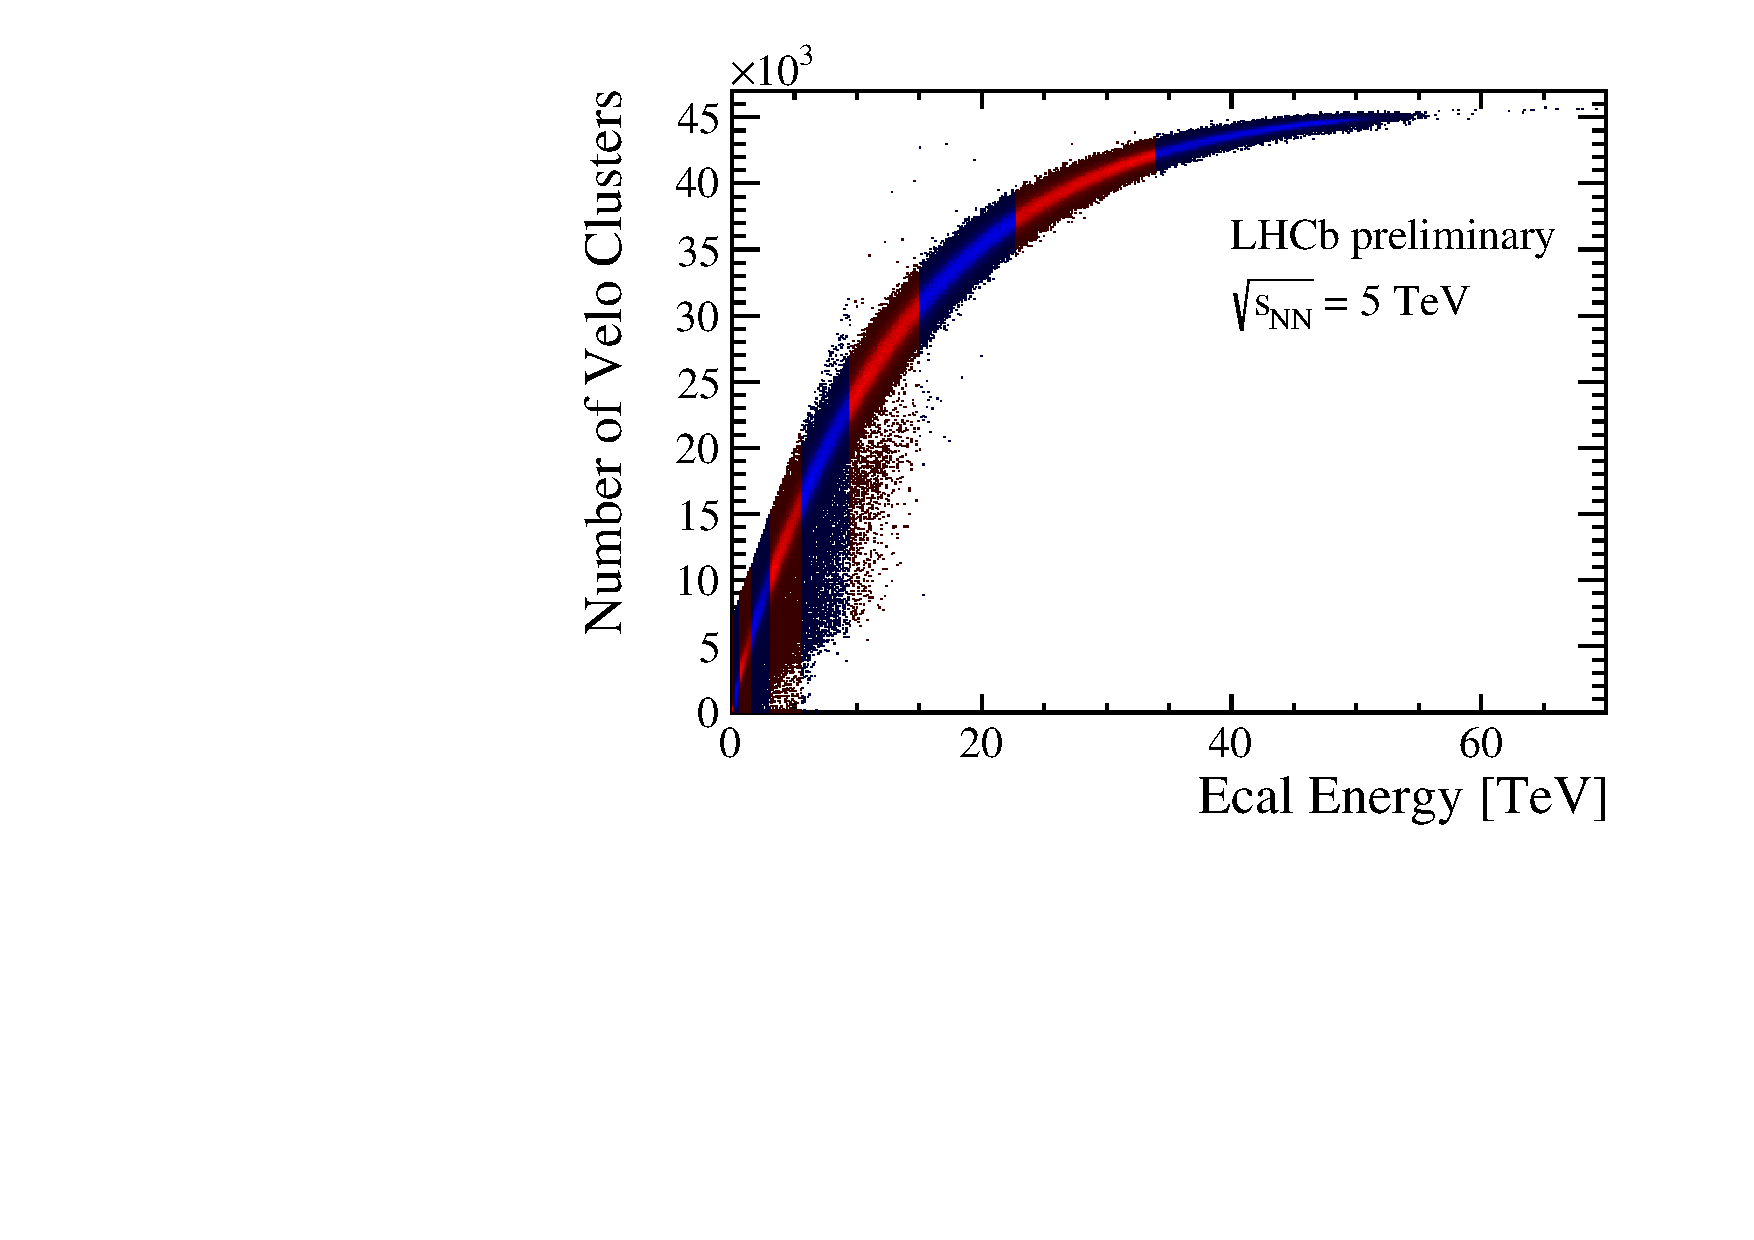
\includegraphics[width=0.48\textwidth]{plots/velo_vs_ecal.pdf}
%   \end{center}
%   \caption{Number of VELO clusters as a function of the calorimeter energy. Colors represent different centrality classes.}
% \end{wrapfigure}

\begin{figure}[htb]
  \begin{center}
    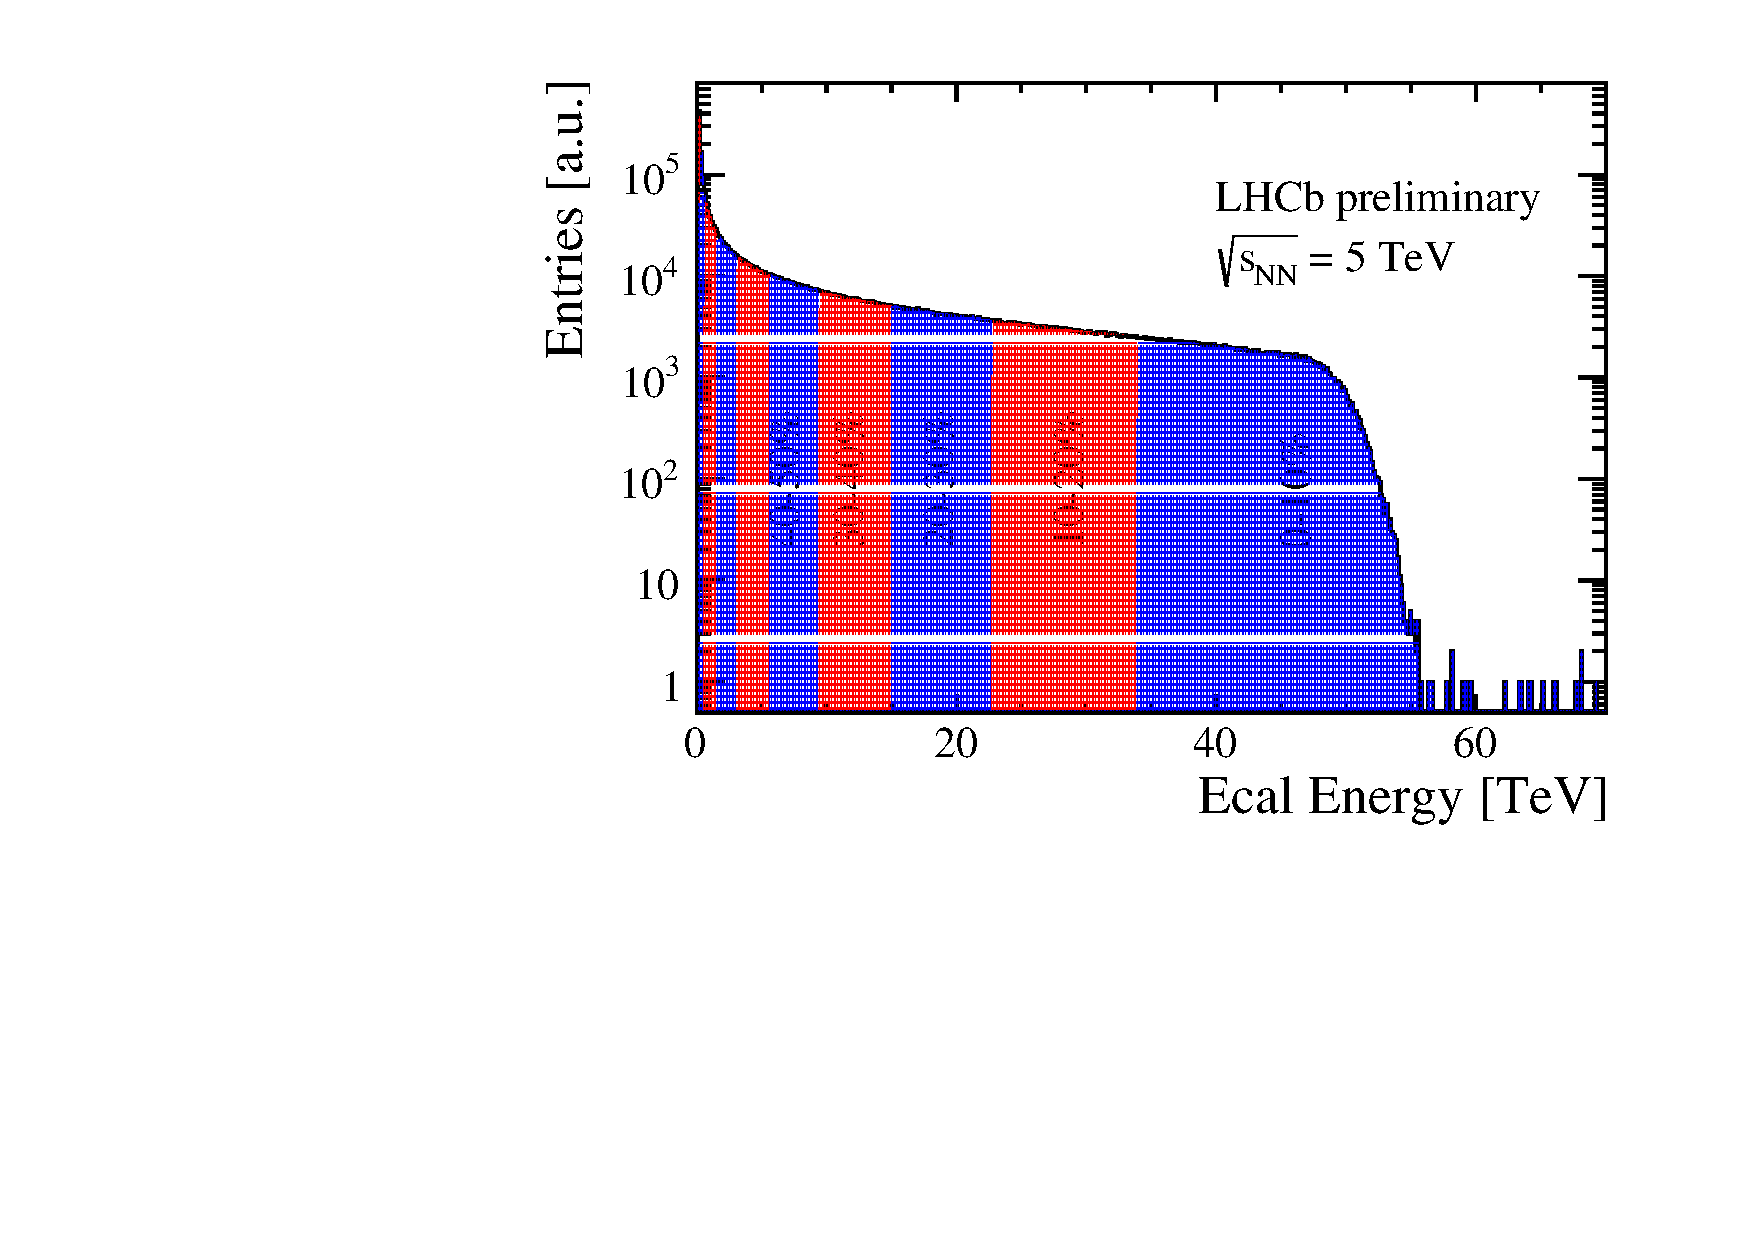
\includegraphics[width=0.48\textwidth]{plots/ecal_in_ecal_bins.pdf}
    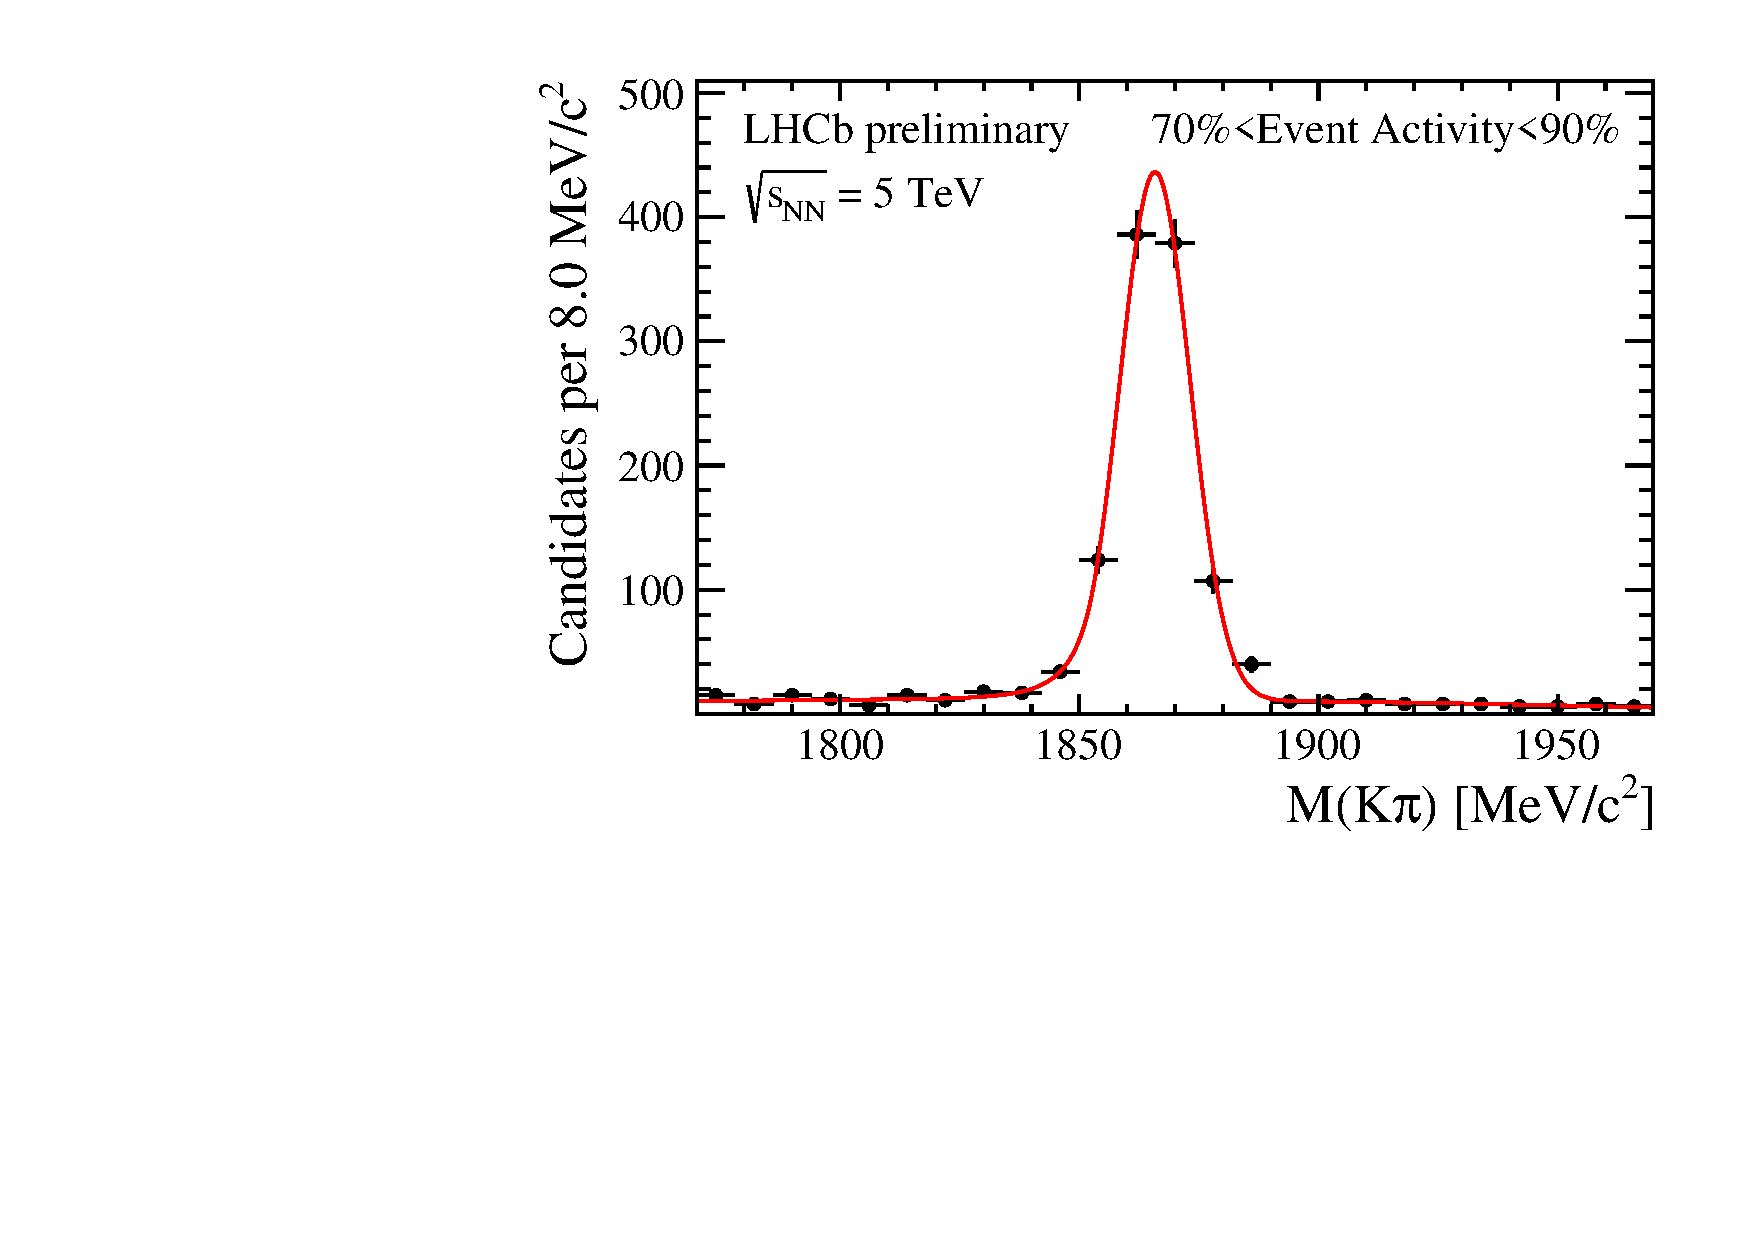
\includegraphics[width=0.48\textwidth]{plots/d0_ecalbin_90_70.pdf}
%     https://twiki.cern.ch/twiki/bin/view/LHCb/LHCbPlots2015
  \end{center}
  \caption{Left: Electromagnetic calorimeter energy distribution in 
PbPb collisions divided into centrality classes highlighted in different colours.
  Right: $\Dz \to \K\pi$ in 70-90\% \pbpb in LHCb. 
  \label{fig:pbpblhcb}}
\end{figure}

LHCb also features a System for Measuring the Overlap with Gas (SMOG), consisting in the injection of a noble gas at very low pressure in the VELO, to measure the beam
position and profile with very high precision. It also allows for the study of the collision of the proton or Pb-ion LHC beam with the gas, in a ``fixed target'' mode.
The corresponding rich physics program, beyond the scope of this project, does not suffer from the tracking limitations exposed above, thanks to the smaller track multiplicity
at these much smaller centre-of-mass energies.


\subsubsection{Overview of the action}

The project will focus on heavy flavour measurements in heavy ion collisions with the LHCb experiment. $\Upsilon$ mesons will be measured in \pPb collisions (to be recorded at the end of 2016), with the expectation to measure the \rpa of the \PgUc meson for the first time in the forward acceptance of LHCb.
\Dz and \Jpsi mesons will also be measured in \pbpb collisions (2018 data). In the case of these charmed mesons, the contributions of prompt and nonprompt production will be distinguished, for the first time
down to null \pt in the forward acceptance of LHCb. The analysis of \pbpb data will require a significant improvement of the tracking algorithms available, so that more
central events can be reconstructed. This will also have a major impact on the LHCb heavy-ion program and open a new physics case for the experiment with the access
to central \pbpb collisions.


\subsubsection{Objectives, research methodology and approach}\label{sec:objectives}

\begin{figure}[htb]
  \begin{center}
    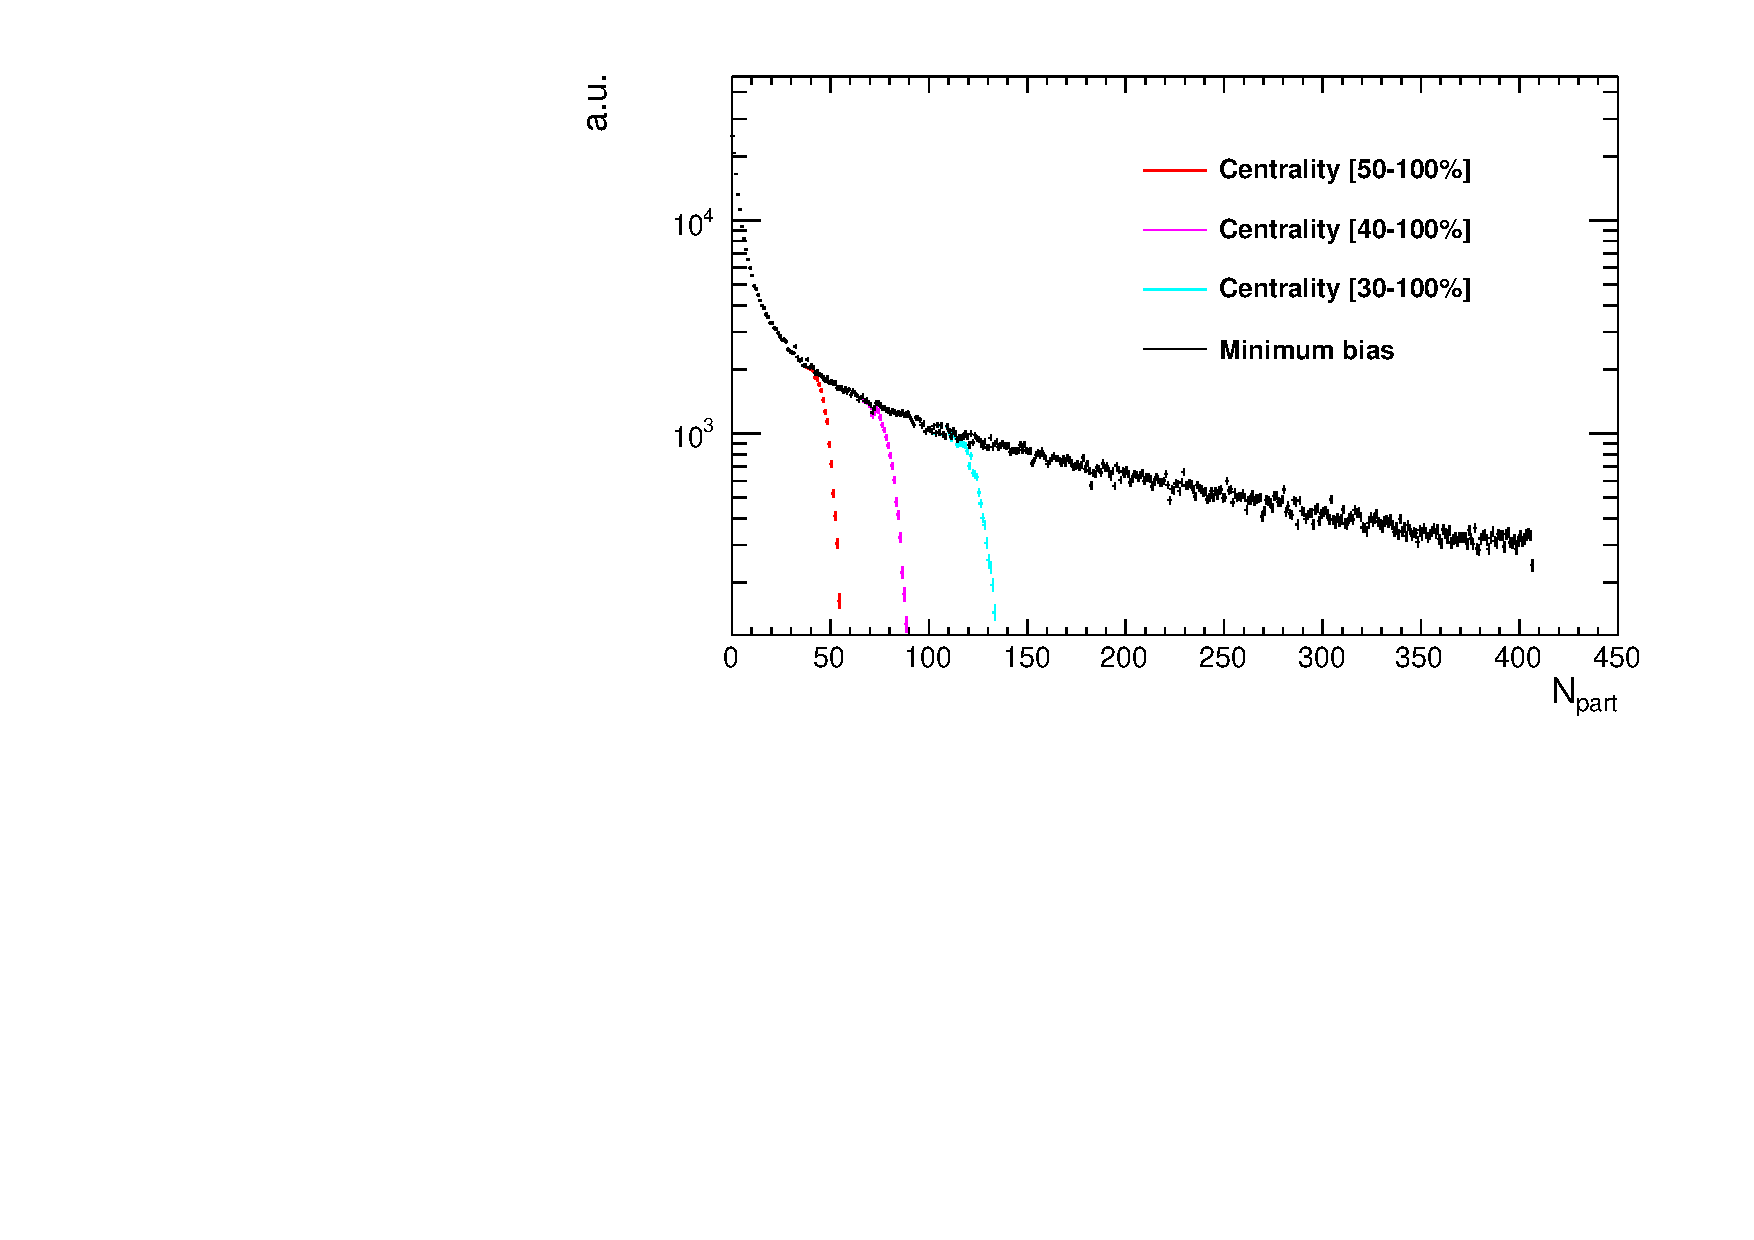
\includegraphics[width=0.4\textwidth]{plots/centrality.pdf}
    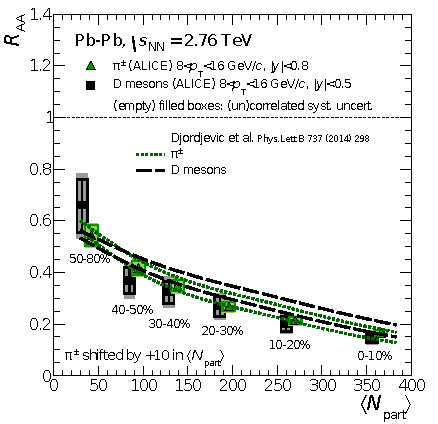
\includegraphics[width=0.28\textwidth]{plots/ALICE_D0.pdf}
    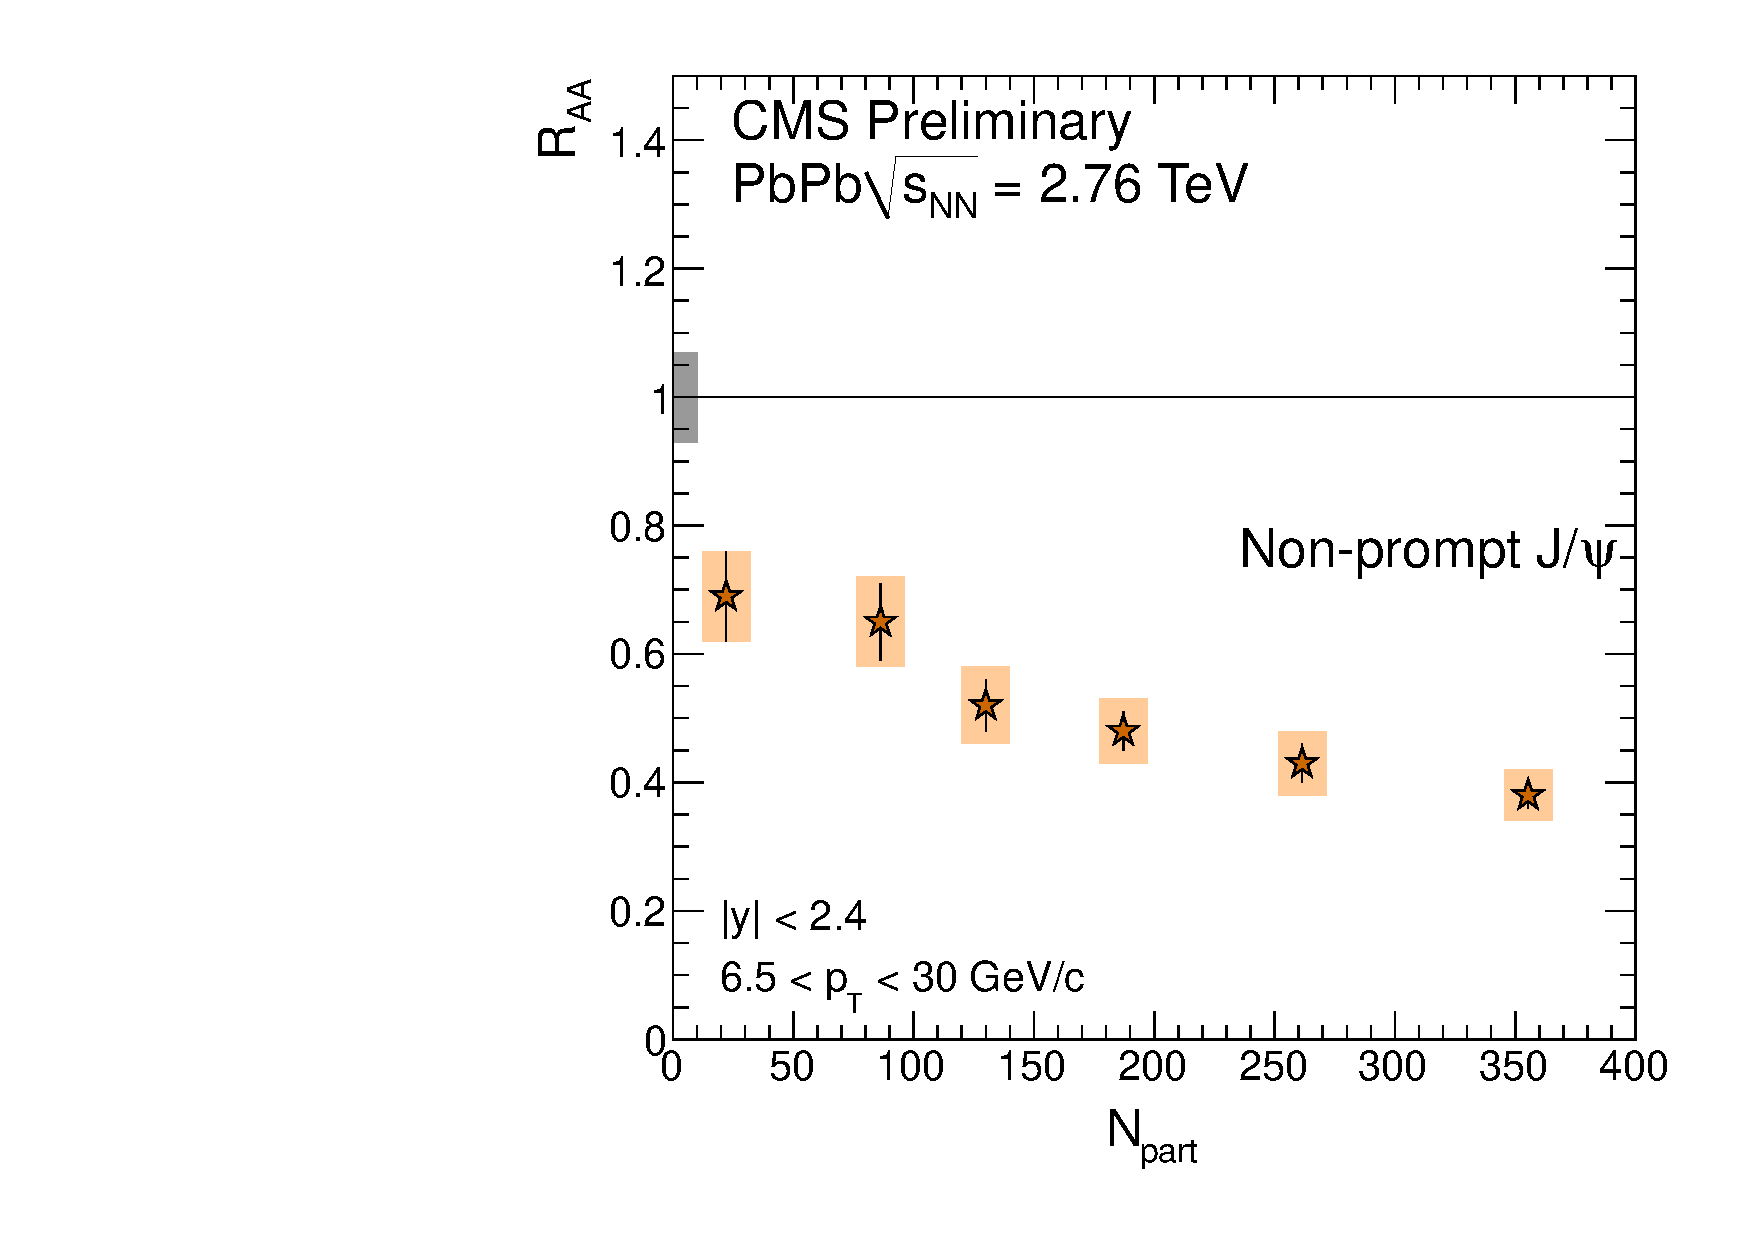
\includegraphics[width=0.28\textwidth]{plots/NonPromptJpsi_RAAvsCent_slides.pdf}
%     https://twiki.cern.ch/twiki/bin/view/LHCb/LHCbPlots2015
  \end{center}
  \caption{Left: \npart distribution (from Hydjet simulation at $\sqrtsnn = 5.02\,\TeV$) with different centrality cuts. Middle: $\raa(\D)$ from ALICE. Right: \raa of nonprompt \Jpsi from CMS.
  \label{fig:npart}}
\end{figure}

\paragraph{Tracking in central \pbpb events. }\ 
The first objective is to be able to reconstruct central events in LHCb. Currently the experiment is only capable of reconstructing events down to approximately 60\% centrality, due to the too high cluster multiplicity in the VELO: it misses most of the hard probe cross sections (which scales as the number of collisions \ncoll rather than the number of participants \npart). This is a major stake in the LHCb \pbpb program: if this limitation would be diminished or removed, LHCb would be able to perform the same physics program in \pbpb as the other LHC experiments, in particular the ALICE muon arm which covers a similar rapidity range. LHCb already benefits from its outstanding performance in terms of particle identification, momentum resolution and access to low \pt particles. A realistic goal would be to push the tracking up to 20\,000 VELO clusters, corresponding to about 30--40\% centrality.

In order to achieve this objective, two main paths will be followed, defined in discussion with LHCb tracking experts. The \ER will be able to benefit from his knowledge from CMS, having gone through the same kind of exercise over the past years. Indeed, he has optimised the Regional Iterative Tracking (RegIt), used to enhance the tracking efficiency in \pbpb in a region around reconstructed muons. For this, he has familiarised himself with the tracking algorithms used in CMS, and their difference between \pp and \pbpb.

\begin{wrapfigure}{r}{0.5\textwidth}
  \begin{center}
    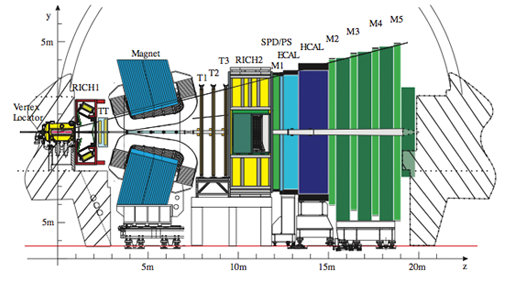
\includegraphics[width=0.5\textwidth]{plots/lhcblayout.png}
  \end{center}
  \caption{The LHCb detector, including the Vertex Locator (VELO), and the Trigger Tracking (TT), Tracking (T) and Muon (M) stations. \label{fig:lhcb}}
\end{wrapfigure}

First, a simplified tracking will be developed, that could be run within the reach of the available computing resources, in terms of time and memory usage. It is crucial to reduce the number of seeds to be considered by the tracking algorithms. For this, the idea would be to tighten the minimum number of clusters in 
the VELO or tracking stations during the pattern recognition (i.e. the track building state). 
% Quality cuts on the track seeds will be tightened, such as the minimum number of clusters in the VELO or in the tracking stations, or the ``ghost probability'' (a variable gauging the likelihood that a track candidate is a fake). 
The goal is to restrict to the best quality seeds, so that the combinatorics of patter recognition is kept at a manageable level in the very high track multiplicity of PbPb collisions, even if that means slightly loosing in terms of track efficiency, especially at very low \pt. In that regard, it would also be possible to reduce the size of the search window used in pattern recognition: this would speed up reconstruction but restrict to straighter (i.e. higher \pt) tracks.

Second, the information from the muon stations can be used, in different ways. Muon tracks can be used as seeds and propagated back through the tracking stations (T, see Fig.~\ref{fig:lhcb}), which will allow for smaller search windows (and ignoring the rest of the detector), compared to starting with no seed at all. The other possible (and complementary) strategy is to match VELO tracks to muon tracks, thus bypassing the T stations, which suffer much more from the high occupancy than the muon stations. Here the idea is to have a higher efficiency for muons, which have a much smaller multiplicity than charged particles in general and are used for measurements involving quarkonia, for instance. 

The \ER will work on these improvements at the same time as getting familiar with the LHCb reconstruction software. Once finalised, he will propose the inclusion of his algorithms in the official LHCb reconstruction software and perform its validation on 2015 \pbpb data and simulation.


\paragraph{\pPb data analysis: \PgUabc. }\ 
The project also involves data analysis of the \pPb data to be taken in November 2016, at $\sqrtsnn = 8\,\TeV$. The measurement of the nuclear modification factor of upsilon mesons, $\rpa (\PgUabc)$, will be performed as it is one of the high profile analyses that can be achieved. LHCb benefits from its excellent dimuon mass resolution ($\lesssim 0.5\%$ for $\pt < 100\,\GeVc$), % 11.55MeV for the J/psi according to p84 of https://cds.cern.ch/record/2202169/files/CERN-THESIS-2012-428_2.pdf
better than any other LHC experiment (and in particular than ALICE in the same rapidity region, $\sim 2.4\%$). %73MeV at the jpsi peak
The measurement of the same quantity by LHCb with 2013 \pPb data at $\sqrtsnn = 5\,\TeV$ will serve as a baseline for this data analysis. Significant improvements will be possible. First, the collision energy of $\sqrtsnn = 8\,\TeV$ will allow to use the large \pp reference dataset available at the same centre-of-mass energy, allowing for a precise mapping of the $\Upsilon$ mesons modification without having to interpolate results at other energies as had to be done with 2013 \pPb data\footnote{LHCb Collaboration,
  %``Study of $\Upsilon$ production and cold nuclear matter effects in $p$Pb collisions at $\sqrt{s_{NN}}$=5 TeV,''
  JHEP {\bf 1407} (2014) 094.
%   doi:10.1007/JHEP07(2014)094
%   [arXiv:1405.5152 [nucl-ex]].
  }.
Second, the much larger dataset (1.6\,\nbinv in 2013, 20\,\nbinv expected in 2016) will allow a much more precise measurement, including the access to the \PgUc (whose \rpa has never been measured so far).

The \ER will lead the effort on this data analysis, being the contact person for the LHCb Collaboration. He will be involved in all parts of the analysis, from defining the selection to evaluating the efficiencies in simulation, producing the results and bringing them to publication. He will receive the help from a PhD student which he will supervise.


\paragraph{\pbpb data analysis: \Dz and \Jpsi. }\ 
Heavy flavour physics will also be investigated in \pbpb data, taking at the same time the opportunity to profit from the improved tracking algorithms to be developed for \pbpb as mentioned above. 

First, the nuclear modification factor of \Dz mesons will be measured, in the $\Dz \to \K\pi$. The same analysis techniques as used in \pPb\footnote{LHCb Collaboration, LHCb-CONF-2016-003.} will be adapted for \pbpb. Similar \Dz meson measurements are available from the ALICE and CMS experiments, but at central rapidity and, most of all, not down to 0 \pt, which only LHCb has the possibility to do. The absence of any \pt threshold is crucial as it gives direct access to the full cross section. The possibility to separate
prompt \Dz mesons from those coming from B meson decays will also be a key ingredient, giving access to an unambiguous measurement of the prompt \Dz as well as an access to the \raa
of B mesons.

Similarly, the \raa of \Jpsi will be measured, separately for prompt and nonprompt \Jpsi, again with a unique access to 0 \pt (ALICE has access to 0 \pt \Jpsi but cannot separate prompt from nonprompt \Jpsi; CMS can make the latter separation but with a \pt threshold of 3\,\GeVc). The experience of the \ER with \Jpsi measurements in \pbpb
in CMS will be of key importance. The nonprompt measurements from the \Dz and \Jpsi, arising from the same physics (modification of B mesons in \pbpb), will be compared. The comparison of the \raa of the \pt-inclusive prompt \Jpsi and \Dz, i.e. of hidden to open charm, is also of primary interest as recently underlined\footnote{H. Satz. In: Adv. High Energy Phys. 242918 (2013).}.

Both the \Dz and \Jpsi analyses will both be first performed using 2015 \pbpb data, re-reconstructed using the improved tracking algorithms developed in the scope of this project. They will then be published using the 2018 data, at the same collision energy but an expected two to ten times higher statistics. The exact involvement of the \ER in these analyses, which require the improved tracking in \pbpb, will depend on the exact time needed by the latter. He will naturally focus in priority on aspects of the analysis directly related to tracking, such as the selection (quality and kinematic cuts) as well as the efficiencies.


\subsubsection{Originality and innovation aspects of the research programme}

The design of dedicated and specially optimised tracking algorithms for the reconstruction of \pbpb collisions with LHCb will be a major breakthrough for the LHCb experiment. This will require the development of novel experimental strategies, but the \ER will be able to base on his knowledge of the specificities of tracking for \pbpb collisions in CMS.

This optimised tracking will then be used for the measurement of \Dz and \Jpsi mesons in \pbpb data, taking advantage of the strengths of LHCb compared to other LHC experiments: access down to 0 \pt, excellent momentum resolution (sharp resonances and good signal significance over the continuous background), excellent impact parameter resolution (for separation of the prompt and nonprompt components).

The measurement of \PgUabc in \ppb collisions will also benefit from these features of the LHCb detector. Besides the excellent precision of the measurement, it should present the \rpa of \PgUc for the first time, which would be crucial in disentangling CNM from QGP effects.

The contents of this proposal are currently not covered in LHCb. It would allow to go beyond the scope of \supervisor's ERC project. In particular, it is a unique opportunity to reach more central \pbpb events with LHCb, and the novel tracking algorithms developed will be used in data analysis, for \Dz and nonprompt \Jpsi, allowing to roughly double the current \npart reach of data analyses in LHCb. 
% 
% 
% \begin{itemize}
%  \item Improvement of tracking in PbPb in LHCb: crucial to the physics program
%  \item Upsilons in pPb: potential for unprecented precision, excited states. Baseline = $R_{pA}$ / $R_{FB}$
%  \item Other analysis... using the brand new PbPb tracking. 
% \end{itemize}

% \subsubsection{Gender dimension} % removed after a comment from Alessia
% 
% The \ER is male but \supervisor is female, and INFN includes about 15\% women, a number which is constantly increasing also thanks to the action of the ``Early Career and Gender Diversity Committee'' recently created at LHCb. 

\subsubsection{Interdisciplinarity}

This project's scope is limited to physics. Nevertheless, it will connect different fields of physics, as it will open a new physics case in a LHCb, fully enabling heavy-ion physics in an experiment originally designed for b-physics.
% It relates two communities that are usually quite disconnected, focusing on in-medium QCD (heavy ion collisions) and in-vacuum standard model (proton-proton collisions).  The \ER is used to bridge the two, having worked both on Higgs and QGP physics (the latter in a multi-purpose experiment), as is the host, who has also worked in CDF and LHCb. This project will significantly enhance the physics case of the LHCb experiment (originally primarily focused on B physics) in the study of heavy ion collisions. 
In addition, there will also be the possibility to perform a phenomenology interpretation of some of the measurements performed within this project (e.g. the $\rpa(\PgUabc)$), especially given the \ER's interest in this regard. Such a study could be performed together with the \ER's past collaborators and / or with the theory group of the host institution. \Supervisor is involved in a project with the theory and ALICE  groups in Cagliari. If funded, this would lead to a new collaboration based on the study of new observables indicated by the theorists which could shed light on the very nature of QGP.

%   _       ___ 
%  / |     |_  )
%  | |  _   / / 
%  |_| (_) /___|
%       

\subsection{Clarity and quality of transfer of knowledge/training}

% {\tiny
% Describe the training that will be offered. \\
% Outline how a two way transfer of knowledge will occur between the researcher and the host institution(s):
% \begin{itemize}
%  \item Explain how the experienced researcher will gain new knowledge during the fellowship at the hosting organisation(s)
%  \item Outline the previously acquired knowledge and skills that the researcher will transfer to the host organisation(s).
% \end{itemize}
% }


\subsubsection{Benefit for the applicant}
\label{sec:benefitapplicant}

The \ER will learn new skills regarding tracking, on top of his knowledge from CMS, for a new detector and having to develop the fundamentals of new algorithms. More generally speaking, his move to a new Collaboration, from CMS to LHCb, will require that he learns about a new environment, new software, and new detector (with a different architecture from a general purpose detector such as \DO or CMS). 

Among the specificities of LHCb, he will learn about particle identification (PID, the convener of this group is at INFN Cagliari) and its use in data analysis, e.g. for the \Dz in \pbpb analysis. 
% Indeed, the \ER has mostly worked with leptons so far (electrons and muons), and the use of identified charged hadrons for data analysis will be new to him.
This would expand the knowledge of the \ER, who has worked mainly with leptons in the past. Using identified charged hadrons for data analysis would be an important addition to his physics baggage.

% move elsewhere? following is not directly knowledge transfer
% It will be also the first time for the \ER to be settled outside France and to work for a non-French institution, an experience particularly important when working in the large international collaborations that are LHC experiments. 
He will also learn to manage a project of his own, including the associated budget, in particular for travel to CERN and conferences, a situation that he will encounter repeatedly later in his career. The experience of \supervisor with managing projects, including the ERC Consolidator Grant, will be valuable in that sense.

He will improve his communication skills, which will be an important part of the project: communication inside the LHCb Collaboration with internal talks and documents, communication to the community with several papers anticipated, as well as seminars and talks at international workshops and conferences, etc. His involvement in the supervision of a PhD student, into more detail than he has had the occasion until now, will also improve his management skills.

The \ER's scientific network will also be expanded, with connections to a new experiment (LHCb) and a new institution (INFN Cagliari). In this way he will place himself at the heart of the community interested in heavy flavour measurements in heavy ion collisions at the LHC.



\subsubsection{Benefit for the host}

The \ER's knowledge about tracking from CMS, in particular for \pbpb collisions, will be very important for the host when transposed in LHCb: he has been leading the effort on the improvement of RegIt, gaining up to a factor 2 on the reconstruction efficiency for very displaced muons. His experience with working on heavy ions inside a general purpose LHC experiment will also be valuable. More generally, interactions between people from different experiments, with complementary approaches to detector algorithms and data analysis, prove to be a good way to let new ideas emerge. 

The host will also benefit from the \ER's previous network. Besides \supervisor's strong connection with LAL Orsay, but also LLR (through Frédéric Fleuret), the \ER will keep his contacts with the CMS heavy ion groups of LLR but also other institutions. His collaboration with François Arleo, one of the authors of the energy loss model, crucial to the description of heavy flavour especially in \ppb, will also be appreciable.

The INFN Cagliari already has a ALICE and LHCb group (the latter
focusing on pp collisions). A new heavy-ion pole has been created in the
LHCb Italy group, with INFN Florence joining the SMOG activities -- one 
of the heavy ion working group convener in LHCb is from this institute --
and the recent move of \supervisor to Cagliari. The arrival of the 
\ER will extend the activities in the lab and its visibility in
the heavy-ion and LHCb communities as well as creating an
interface with the ALICE and CMS Italian communities.



%   _       ____
%  / |     |__ /
%  | |  _   |_ \
%  |_| (_) |___/
%           

\subsection{Quality of the supervision and the hosting arrangements} 
\label{sec:supervision}

\subsubsection{Qualifications and experience of the supervisor}

% {\tiny
% Provide information regarding the supervisor(s): the level of experience on the research topic proposed and their track record of work, including main international collaborations, as well as the level of experience in supervising researchers. Information provided should include participation in projects, publications, patents and any other relevant results.}
% 

The supervisor (Dr. Giulia Manca) is an associate professor at the 
University of Cagliari and INFN. After graduating with an 
analysis in neutrino physics (CHORUS experiment), she obtained her 
PhD at the University of Oxford, UK, in the CDF experiment at Fermilab,
where she worked in Electroweak physics first and Supersymmetry later
(as post-doc with the University of Liverpool, UK), becoming 
CDF SUSY convener and leading the effort of a team of young scientists
at Fermilab.
After a few months in ATLAS, in 2007 she moved to Cagliari and 
joined the LHCb experiment, where she worked on quarkonia physics, 
becoming sub-convener first and convener after of the related physics groups.
She lead several \Jpsi and \PgU analyses in \pp
collisions, and supervised several post-docs and graduate 
students both at CERN (where she spent two one-year periods
in 2010 and 2012) and at her home institution. In April 2015 she
was awarded a ERC Consolidator Grant to start a heavy ion physics 
programme at LHCb. She moved to Orsay (FR) 
where she started and coordinated a group of three post-docs and 
two senior researchers, who became the leading force of the 
heavy ion physics programme at LHCb. Under \supervisor's 
leadership, LHCb collected for the first time data in \PbPb 
collisions and explored a completely new energy by analysing
data with the ``SMOG'' fixed target setup.
The first analysis of \JPsi production using the \PbPb dataset 
is currently under internal review
and it is expected to be published by the end of 2016. 
In September 2016 \supervisor\ moved to the University of Cagliari and INFN where 
she has started a new group joining the heavy ion LHCb effort within 
the ERC project. The group will consist
of one young post-doc, one PhD student (PhD1) and \supervisor. 
The Cagliari group will work 
in constant collaboration with the Orsay group, which \supervisor\
will lead together with the senior researchers. Regular meetings and 
travel will be organised between the two institutions.
\Supervisor\ is also involved in a local project funded by the 
Sardinian administration, ``Regione Sardegna,'' to address the studies of 
polarisation of charmonium states at the ALICE and LHCb experiments
together with scientists of the ALICE and theory groups in Cagliari.
She is also the responsible of the ``INFN summer student program'' in 
Cagliari and supervised undergraduate students from the 
university of Cincinnati 
and UCLA selected through the program who spent three
months in Cagliari in 2014 and 2015.
\Supervisor is author and co-author of more than 800 
papers published in peer-reviewed journals, more than 100 of which 
in the field of interest for the project, and has an ``H-index'' of 86.
She has tutored several Master Degree and PhD students and has
 been part or chair of several national
and international scientific committees and thesis juries.



\subsubsection{The Host}

% {\tiny
% The application must show that the experienced researcher will be well integrated within the team/institution in order that all parties gain the maximum knowledge and skills from the fellowship. The nature and the quality of the research group/environment as a whole should be outlined, together with the measures taken to integrate the researcher in the different areas of expertise, disciplines, and international networking opportunities that the host could offer. }

The research group in Cagliari
will be the perfect fit where to nicely integrate the \ER, from the
personal and professional point of view. 
The LHCb Cagliari group has a long expertise in 
muons both from the hardware and software 
aspects, having among his members the Muon 
detector project leader and the convener of the 
% Particle Identification
PID LHCb group.

The members hired on the 
ERC grant will 
concentrate on the completion of the \JPsi analysis of the 
\PbPb dataset in peripheral events together with \supervisor\ and the 
Orsay group. The current 
version of these analyses indicate that the 
poor performance of the PID and tracking algorithms at high occupancy 
(thus low centrality) is the main limitation already 
in the centrality of 60-70\%. The ERC post-doc and the student will 
concentrate on the adaptation of the PID criteria
for muons and hadrons in the busy \PbPb environment.
In this they will benefit by the collaboration 
with the PID convener in 
Cagliari, who has great expertise in this area.
If awarded the grant, the \ER will start the development of 
new tracking algorithms to perform efficiently in higher 
occupancy events whose analysis is not included in the ERC project.
These studies, complementary to the ones supported by the 
ERC grant, will be crucial as they will extend the 
reach of LHCb in PbPb analyses as well as consolidate 
its impact in the field.
The University of Cagliari will provide a PhD student position (PhD2) 
independent on the ERC grant who would work closely with the 
\ER and \supervisor on the subjects of the proposal.
Since LHCb is relatively new in the 
heavy ion physics community, the experiment
will profit enormously from the experience 
of the \ER who has pioneered the heavy-ion physics 
in CMS when only a few scientists started working 
in this area. 
The expertise the \ER has developed in the CMS 
heavy ion community would be crucial to 
realise the huge potential of LHCb in this field.

The \ER, with long-lasting experience in heavy nuclei
collisions and large collaborations, commissioning
of a new physics stream, optimization and simulation, data analysis and track
reconstruction, will nicely complement the activities
of the new group and will in
in particular coordinate the 
collaboration with the 
theory group in Cagliari, as he has 
done successfully in the past.


The experience of the other INFN 
researchers in the group will be a very important addition to the \ER's
education and will contribute to his development as independent
researcher. At the same time, being in an already established research
group will give the \ER a better chance to pass on his previously
acquired knowledge and skills to the INFN scientific community. 
The international background of \supervisor and her 
broad physics experience will ensure that the 
\ER will be inserted in a international network of 
research groups around the world.  
\Supervisor and the \ER will draw together a Career Development Plan,
with the major accomplishments expected from this research project in
light of short-term and long-term career objectives. Fortnightly
meetings will be held between \Supervisor and the \ER to monitor the
advancement and define the strategy, in order to take proper actions
to fulfil the deadlines. Thanks to the INFN long-lasting tradition of
international training schools, the \ER will also have the chance to take
part to various kind of training courses in order to improve his
skills and know-how.  

%   _       _ _  
%  / |     | | | 
%  | |  _  |_  _|
%  |_| (_)   |_| 
%              
            

\subsection{Capacity of the researcher to reach and re-enforce a position of professional maturity in research}
\label{sec:maturity}
% {\tiny
% Applicants should demonstrate how the proposed research and training will contribute to the further professional development as an independent/mature researcher.  \\
% Describe briefly how the host will contribute to the advancement of the researcher's career. \\
% Therefore, a complete Career Development Plan should not be included in the proposal, but it is part of implementing the action in line with the European Charter for Researchers.\\}

The \ER has gained a position of expertise in several complementary areas. He has had a leading contribution to analysis of proton-antiproton data (with \DO), proton-lead and lead-lead data (with CMS), on physics topics ranging from Higgs boson searches and anomalous quartic gauge couplings (aQGC) in photon interactions to nuclear parton distribution functions (nPDF) and quarkonia. His prominent role in the CMS heavy-ion group has lead him to be appointed convener of the dilepton Physics Interest Group (PInG), counting 20 people from 7 institutions and 3 continents and gathering physicists interested in electroweak and quarkonium physics in HIC in the Collaboration.

At the same time, he has also showed interest in phenomenology, having co-signed to phenomenological papers, on aQGC and W boson production in hadronic collisions. The second article was co-signed with François Arleo, whose energy loss model for quarkonium production in HIC is one of the most predictive on the market, and Hannu Paukkunen, co-author of the most used nPDF set, EPS09. This connection could be useful in interpreting in depth upsilon production in pPb collisions, where both nPDF and energy loss are key ingredients to the modification with respect to \pp collisions.

The \ER is also responsible for muon reconstruction in HIC in CMS,
having lead the effort on the improvement of RegIt. But while the
algorithm was already existing in CMS, he will have to work on deep
modifications of the tracking algorithms with the LHCb experiment, a
great way to try and transpose CMS' approach of outside-in tracking
from the muon systems and to improve his skills in this domain. In 
LHCb the \ER will be the first one to design and develop these new
techniques supported by the supervisor. He will start the effort, define 
the methodology and coordinate the work of the PhD student (PhD2) and other 
post-docs potentially joining from different LHCb institutions.
This will bring him to be recognised as the responsible and leader 
of this effort
in LHCb, bringing a major and visible contribution to the experiment.

This project will also help the \ER strengthen his management skills, essential to his maturity in research. He will be involved in the supervision of PhD2 on the \rpa of \PgUabc. He will also have to support his \pbpb tracking in the LHCb collaboration, in discussion with the software and detector experts. He will 
% have the opportunity to take part to the organisation of mini-workshops in INFN Cagliari, a new activity to him.
have a leading role in the interactions with the theorists in Cagliari, strengthening the interdisciplinarity of the project. The \ER will also be actively involved in the organisation of a workshop in 2018 where he will present his 
results. This is an activity new to him where he could profit from the 
expertise of \supervisor and the colleagues at the host institution, which 
have a long tradition in this area.

%   ___     
%  |_  )    
%   / /   _ 
%  /___| (_)
%           

\section{IMPACT}
\label{sec:impact}

%   ___       _ 
%  |_  )     / |
%   / /   _  | |
%  /___| (_) |_|
%               

\subsection{Enhancing the potential and future career prospects of the researcher }
\label{sec:enhancement}
% {\tiny
% Explain the expected impact of the planned research and training on the career prospects of the experienced researcher after the fellowship. Which new competences will be acquired?}

This project will bring considerable new knowledge and experience to the \ER, as exposed in Sections~\ref{sec:benefitapplicant} and \ref{sec:maturity}. Besides, both quarkonium physics and tracking are in phase with the interests of the French heavy-ion community. Quarkonium production in HIC has been studied in several laboratories, in all 3 LHC experiments represented in France for HIC: ALICE, CMS and LHCb. 
The experience gained by the applicant in LHCb would be extremely valuable
also if the \ER would decide in the future to join the ALICE experiment, which 
covers a similar region in rapidity. This could open new routes to the \ER 
in countries like Germany, with a strong ALICE and heavy ion theory community.

Regarding tracking, several of the CMS experts in tracking in HIC work or have worked at LLR, and France is deeply involved in the Muon Forward Tracker upgrade for ALICE, requiring combined tracking with the muon chambers. \Supervisor has started her ERC project at LAL Orsay, and keeps a tight collaboration with this group, sharing the same interests inside the LHCb heavy ion community. This collaboration will be profitable for the project, and regular travel to LAL is anticipated. Thus, this project will allow the \ER to develop a very valuable experience in view of obtaining a permanent position in Europe, which is the next step in his career.



%   ___       ___ 
%  |_  )     |_  )
%   / /   _   / / 
%  /___| (_) /___|
%                

\subsection{Quality of the proposed measures to exploit and disseminate the action results }

% {\tiny
% Describe how the new knowledge generated by the action will be disseminated and exploited, e.g. communicated, transferred into other research settings or, if appropriate, commercialised. 
% 
% What is the dissemination strategy - targeted at scientists, potential users and to the wider research and innovation community - to achieve the potential impact of the action? \\
% Please make also reference to the "Dissemination \& exploitation" section of the H2020 Online Manual1. \\
% The following section of the European Charter for Researchers refers specifically to dissemination:\\
% \textbf{Dissemination, exploitation of results}\\
% All researchers should ensure, in compliance with their contractual arrangements, that the results of their research are disseminated and exploited, e.g. communicated, transferred into other research settings or, if appropriate, commercialised. Senior researchers, in particular, are expected to take a lead in ensuring that research is fruitful and that results are either exploited commercially or made accessible to the public (or both) whenever the opportunity arises. \\
% Concrete planning for section 2.2 must be included in the Gantt Chart (see point 3.1). \\
% }

% The new tracking algorithms will be beneficial to the whole HIC group of LHCb, giving access to more central events. 

First, the results from the proposal will be discussed inside the
Cagliari group, as well as in regular mini-workshops at Cagliari, 
between the theory, ALICE and LHCb groups which the \ER will
help organising. The results will also be
spread inside the LHCb collaboration, being presented at internal
meetings (tracking and heavy ion physics). The new tracking algorithms
in particular will be developed, validated and advertised with the
LHCb tracking experts. They could also lead to a technical publication
(for a journal such as Nuclear Instrumentation Methods), describing
the novel algorithms developed, to be cited in all subsequent LHCb
physics publications using this new tracking. The physics results
themselves will be published in high-impact journals, most likely
Physical Review Letters since they involve first-time
measurements. The \ER will present the results in the main conferences in the
field, such as Quark Matter or Hard Probes. Given
the small size of the heavy-ion group in LHCb, participation to these
major conferences will be easier than in other experiments. For the
same reason, the \ER will quickly gain a very high visibility, both
inside the LHCb collaboration and within the heavy-ion community.
Given the huge contribution given by the \ER to the understanding of the 
first PbPb data, by the end of his fellowship the \ER will be in the 
ideal position to analyse the PbPb dataset which will be collected
at the end of 2018, opening new possibilities for his 
career. 



%   ___       ____
%  |_  )     |__ /
%   / /   _   |_ \
%  /___| (_) |___/
%           

\subsection{Quality of the proposed measures to communicate the action activities to different target audiences }
% 
% {\tiny
% Please make also reference to the guidelines Communicating EU research and innovation guidance for project participants1 as well as to the "communication" section of the H2020 Online Manual2.
% Concrete planning for section 2.3 must be included in the Gantt Chart (see point 3.1). 
% 
% The following section of the European Charter for Researchers refers specifically to public engagement:\\
% \textbf{Public engagement}\\
% Researchers should ensure that their research activities are made known to society at large in such a way that they can be understood by non-specialists, thereby improving the public's understanding of science. Direct engagement with the public will help researchers to better understand public interest in priorities for science and technology and also the public's concerns. \\}

The \ER will be involved into events for communication to a general
audience, already organized by the host institute. This includes
outreach seminars in schools, and the yearly organisation of master
classes for high school students, on physics topics including heavy
ions, which are held at the INFN Cagliari site.  Besides, INFN organises 
national yearly events as the ``European research night'', where researchers
in Cagliari as in many other Italian cities organise activities and guided tours of the 
physics department and the museum as well as the 
astrophysics observatory until midnight.
A week-long science festival is also organised in Cagliari every year, 
with the strong participation of INFN Cagliari on general particle physics 
items. The \ER could prepare the heavy ion information for the general public together with the 
ALICE colleagues, and participate to the illustrative tours of the INFN
facilities and laboratories taken in turns 
by INFN personnel. 
Open days are also organised at INFN Cagliari every year, inviting schools and
public to visit the laboratory and the museum and listen to seminars.
The \ER will be trained as a guide for the physics museum, which 
is part of the Physics department and will be able to lead regular 
visits from schools of all Sardinia.
%   ____    
%  |__ /    
%   |_ \  _ 
%  |___/ (_)
%        

\section{IMPLEMENTATION}
\label{sec:implementation}

%   ____      _ 
%  |__ /     / |
%   |_ \  _  | |
%  |___/ (_) |_|
%            
           
\subsection{Coherence and effectiveness of the work plan}

In the first year of the project the \ER could perform studies of \PgU
production with the proton-lead sample which will be collected at the
end of 2016. In this respect the \ER could profit from collaborating
with \supervisor who has large expertise with the \PgU analysis at
LHCb. Since event occupancies are expected to be lower in \pPb than in
\PbPb, this sample will be the ideal complement to the existing \PbPb
sample collected in 2015 and the \JPsi and \psiP activities
supported by the ERC grant, as it has fewer challenges and larger
statistics. The \ER could work with a PhD student on this analysis,
thus refining his tutoring skills which can be pivotal in reaching the
maturity for a teaching position.  The analysis of the three \PgUn
states in \pPb data will be essential to establish the observation of
the suppression of this state, and disentangle CNM from QGP effects.
Once tested on \pPb data, the \ER will be able to apply the new
technique to the \PbPb data.  LHCb is the only active experiment able
to separate the prompt from the delayed component without any \pt threshold at forward rapidity, thanks to the superb
performance of the LHCb detector. Its capability to go down to zero
transverse momentum in the open charm studies, which has already been
proved in the pPb dataset, would be the other completely unique
feature of LHCb in heavy nuclei collisions. Unfortunately, at the
moment LHCb had to limit itself to the analysis of peripheral events
due to the limitations of the tracking. Thanks to the new tracking
strategy developed by the \ER, LHCb would be able to expand the
physics reach to more central collisions, thus being directly
competitive with the ALICE experiment in the same rapidity range. The
impact of the work of the \ER in this field would be enormous for the
LHCb experiment and for the physics community, and will contribute to
the categorisation of the QGP.

\subsubsection*{Work Packages description}

\textbf{This project involves 4 work packages (WP)}, following the list of objectives described in Section~\ref{sec:objectives}. \textbf{\textcolor{red}{WP1}} is the development of tracking algorithms suitable for central events. \textbf{\textcolor{blue}{WP2}} is the measurement of upsilon meson production in \pPb data taken in 2016. \textbf{\textcolor{green!50!black}{WP3}} is the analysis of \pbpb data, using the improved tracking algorithms from WP2. The focus will be the measurement of \Dz and prompt and nonprompt \Jpsi in \pbpb. At last, \textbf{\textcolor{magenta}{WP4}} is the participation to the 2018 \PbPb run.

% \begin{enumerate}
%  \item Development of tracking algorithms suitable for central events
%  \item Measurement of upsilon meson production in \pPb data taken in 2016
%  \item PbPb analysis: \Dz 
%  \item PbPb analysis: prompt and nonprompt \Jpsi
%  \item Participation to the 2018 \PbPb run
% \end{enumerate}

\subsubsection*{List of major deliverables (D) and milestones (M)}

\begin{itemize}
 \item \textcolor{red}{M.1.1} Present preliminary tuned tracking for \pbpb to LHCb tracking experts
 \item \textcolor{red}{D.1.1} Tuned tracking algorithms for \pbpb
 \item \textcolor{red}{D.1.2} \pbpb tracking accounting for the muon information
 \item \textcolor{red}{D.1.3} New \pbpb tracking validated and included in the central LHCb reconstruction software
 \item \textcolor{red}{D.1.4} 2015 data re-reconstructed with the new algorithms
 \item \textcolor{blue}{M.2.1} Start the LHCb internal review of the $\rpa (\PgUn)$ analysis
 \item \textcolor{blue}{D.2.1} Preliminary result on $\rpa (\PgUn)$
 \item \textcolor{blue}{D.2.2} Paper on $\rpa (\PgUn)$
 \item \textcolor{green!50!black}{D.3.1} Definition of the \Dz selection from re-reconstructed 2015 \pbpb data
 \item \textcolor{green!50!black}{D.3.2} Preliminary $\raa(\Dz)$ result on 2018 \pbpb data
 \item \textcolor{green!50!black}{D.3.3} Definition of the \Jpsi selection from re-reconstructed 2015 \pbpb data
 \item \textcolor{green!50!black}{D.3.4} Preliminary $\raa(\Jpsi)$ result on 2018 \pbpb data
 \item \textcolor{magenta}{D.4.1} Trigger strategy for 2018 \pbpb
 \item \textcolor{magenta}{D.4.2} 2018 \pbpb data on tape
\end{itemize}



\begin{figure}[htbp]
\begin{center}
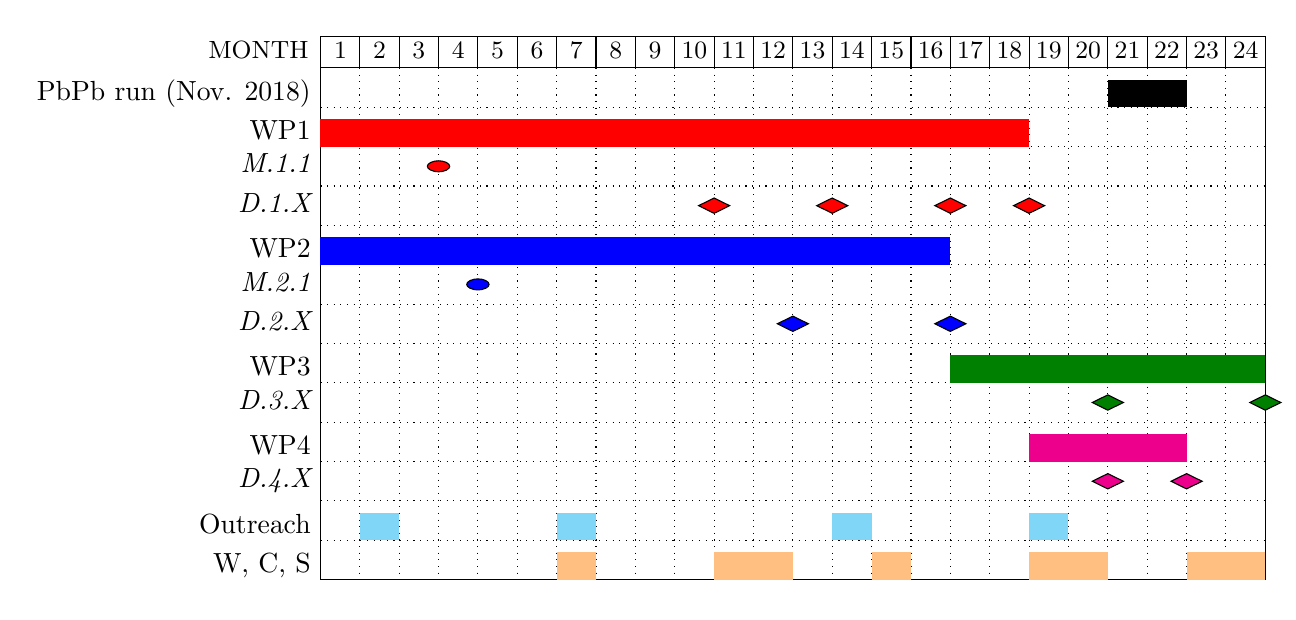
\begin{tikzpicture}[y=0.50cm]  
\begin{ganttchart}[
y unit title=0.4cm,
y unit chart=0.5cm,
vgrid,hgrid, 
title label anchor/.style={below=-1.6ex},
title height=1,
bar/.style={fill=gray!30},
incomplete/.style={fill=black},
progress label text={},
bar height=0.7,
group left shift=0,
group right shift=0,
group height=.6,
group peaks tip position=0,
group label node/.append style={left=.6cm},
group progress label font=\bfseries\small
  ]{1}{24}
  \gantttitle[
    title label node/.append style={left=0pt and -6pt}
  ]{MONTH\quad1}{1}
  \gantttitlelist{2,...,24}{1} \\
%   \gantttitle{2017}{10}
%   \gantttitle{2018}{12}
%   \gantttitle{2019}{2}\\
%   \gantttitlelist{3,...,12}{1} 
%   \gantttitlelist{1,...,12}{1} 
%   \gantttitlelist{1,2}{1} \\
  \ganttbar[bar/.append style={fill=black}]{\pbpb run (Nov. 2018)}{21}{22} \\
  \ganttbar[bar/.append style={fill=red}]{WP1}{1}{18} \\
  \ganttmilestone[milestone/.append style={fill=red, rounded corners=3pt}]{M.1.1}{3} \\
  \ganttmilestone[milestone/.append style={fill=red}]{D.1.X}{10} 
  \ganttmilestone[milestone/.append style={fill=red}]{}{13} 
  \ganttmilestone[milestone/.append style={fill=red}]{}{16} 
  \ganttmilestone[milestone/.append style={fill=red}]{}{18} \\
  \ganttbar[bar/.append style={fill=blue}]{WP2}{1}{16} \\
  \ganttmilestone[milestone/.append style={fill=blue, rounded corners=3pt}]{M.2.1}{4} \\
  \ganttmilestone[milestone/.append style={fill=blue}]{D.2.X}{12} 
  \ganttmilestone[milestone/.append style={fill=blue}]{}{16} \\
  \ganttbar[bar/.append style={fill=green!50!black}]{WP3}{17}{24} \\
  \ganttmilestone[milestone/.append style={fill=green!50!black}]{D.3.X}{20}
%   \ganttmilestone[milestone/.append style={fill=green!50!black}]{}{24}
%   \ganttmilestone[milestone/.append style={fill=green!50!black}]{}{20}
  \ganttmilestone[milestone/.append style={fill=green!50!black}]{}{24} \\
  \ganttbar[bar/.append style={fill=magenta}]{WP4}{19}{22} \\
  \ganttmilestone[milestone/.append style={fill=magenta}]{D.4.X}{20} 
  \ganttmilestone[milestone/.append style={fill=magenta}]{}{22} \\
  \ganttbar[bar/.append style={fill=cyan!50, dashed}]{Outreach}{2}{2} % open days in April?
  \ganttbar[bar/.append style={fill=cyan!50, dashed}]{}{14}{14} % open days in April?
  \ganttbar[bar/.append style={fill=cyan!50, dashed}]{}{7}{7} % research night in September?
  \ganttbar[bar/.append style={fill=cyan!50, dashed}]{}{19}{19}\\ % research night in September?
  \ganttbar[bar/.append style={fill=orange!50}]{W, C, S}{7}{7} % Cagliari mini-workshop
  \ganttbar[bar/.append style={fill=orange!50}]{}{19}{19} % Cagliari mini-workshop
  \ganttbar[bar/.append style={fill=orange!50}]{}{15}{15} % HP??
  \ganttbar[bar/.append style={fill=orange!50}]{}{20}{20} % QM??
  \ganttbar[bar/.append style={fill=orange!50}]{}{11}{12} % seminar marathon for CNRS in January-February :p
  \ganttbar[bar/.append style={fill=orange!50}]{}{23}{24} % seminar marathon for CNRS in January-February :p
%  \ganttbar{Talks for graduate students}{19}{19}
\end{ganttchart}
\end{tikzpicture}
\end{center}

\caption{Gantt chart. The last line (\emph{W, C, S}) stands for \emph{Workshops, conferences, seminars}.\label{fig:gantt}}
\end{figure}


%   ____      ___ 
%  |__ /     |_  )
%   |_ \  _   / / 
%  |___/ (_) /___|
%        


\subsection{Appropriateness of the allocation of tasks and resources }

% Describe how the work planning and the resources mobilised will ensure that the research and training objectives will be reached. \\
% Explain why the amount of person-months is appropriate in relation to the activities proposed.

The project is divided into work packages reflecting its objectives. 
%%FIXME expand

%   ____      ____
%  |__ /     |__ /
%   |_ \  _   |_ \
%  |___/ (_) |___/
%            

\subsection{Appropriateness of the management structure and procedures, including risk management }

% Describe the:
% \begin{itemize}
%  \item Organisation and management structure, as well as the progress monitoring mechanisms put in place, to ensure that objectives are reached;
%  \item Research and/or administrative risks that might endanger reaching the action objectives and the contingency plans to be put in place should risk occur.
% \end{itemize}

\paragraph{Project organisation and management structure: }\
The project will be primarily managed by the \ER, advised by \supervisor. The workflow is embedded in the LHCb
collaboration that has plenty of quality-control procedures. The money will be mostly used by the \ER to travel to
CERN and to conferences, at the \ER’s own choice, validated by \supervisor. There will also be a close collaboration with LAL, where \supervisor started her ERC Consolidator Grant, also needing travel to France. As done in the past,
the money can also be used to invite for short term periods contributors or helpers to the proposed objective and/or
be invested in organizing a workshop.



\paragraph{Risks that might endanger reaching project objectives: }\
The main risk concerns the exact feasibility of reconstructing in good conditions more central events than is currently being done in LHCb. However it would be acceptable to allow for a lower performance of the tracking than in \pp collisions: for instance a lower overall efficiency could be tolerated, especially at low \pt, and / or a higher fake rate. If the \pt threshold in track reconstruction had to be raised too much, the access to 0 \pt \Dz could not be possible in the most central events. It is also unclear what are the most central events that will be accessible. 

There is also the possibility, though very unlikely, that the 2018 \pbpb run would be shortened, postponed or even cancelled, because of issues with the accelerator or the detector, or any other reason. In this case, the project would focus on the analysis of 2015 \pbpb data (despite its much lower integrated luminosity than expected in 2018), already benefiting from the new tracking algorithms developed during the project.

%   ____      _ _  
%  |__ /     | | | 
%   |_ \  _  |_  _|
%  |___/ (_)   |_| 
%      
%      
\subsection{Appropriateness of the institutional environment (infrastructure)}

% The active contribution of the beneficiary to the research and training activities should be described. For GF also the role of partner organisations in Third Countries for the outgoing phase should appear.          
% \begin{itemize}
%  \item Give a description of the main tasks and commitments of the beneficiary and all partner organisations (if applicable).
%  \item Describe the infrastructure, logistics, facilities offered in as far they are necessary for the good implementation of the action. 
% \end{itemize}

%The project will benefit from \supervisor's experience with European projects, including her current Consolidator grant from the European Research Council. The INFN also provides services to help manage such projects.

On the technical side, the INFN Cagliari hosts a large computer cluster which
is shared by the LHCb and ALICE communities. The facility would be
ideal for conveniently and quickly running simulations and data analysis. 
Part of the LHCb Cagliari group is deeply involved in the 
electronics for the LHCb Muon upgrade project, which is 
developed in dedicated equipped laboratories where new chips 
are thought and designed and prototypes are tested. 
Since part of the laboratories are shared with the Cagliari ALICE group,
this vibrant atmosphere would be the ideal place where 
new ideas are developed on possible new experiments 
meant to further the understanding of the very nature of 
QGP. The presence of the Physics museum, unique in Sardinia, 
will allow the \ER to disseminate the knowledge to 
students of all ages from the all region.
\clearpage

%%default options
\titlespacing*{\section} {0pt}{3.5ex plus 1ex minus .2ex}{2.3ex plus .2ex}
\titlespacing*{\subsection} {0pt}{3.25ex plus 1ex minus .2ex}{1.5ex plus .2ex}
\titlespacing*{\subsubsection}{0pt}{3.25ex plus 1ex minus .2ex}{1.5ex plus .2ex}
\titlespacing*{\paragraph} {0pt}{3.25ex plus 1ex minus .2ex}{1em}


\section{CURRICULUM VITAE OF THE EXPERIENCED RESEARCHER}
\label{sec:cv}


\section*{Education}
\begin{tabular}{L!{\VRule}R}
2013&{\bf PhD from Université Pierre et Marie Curie (UPMC, Paris).}\\
2010&{\bf Master: \emph{Noyaux, Particules, Astroparticules, Cosmologie}, UPMC}, ranked first.\\ 
2010&{\bf Diploma from École normale supérieure (ENS) de Cachan}.\\
2007&Bachelor: \emph{PHYTEM (théorie, expérience et modèle)}, UPMC, summa cum laude.\\ %summa cum laude
2006-2010&student at ENS de Cachan, fundamental physics department.\\
% 2004-2006&Classe préparatoire (MPSI - MP$^*$).
\end{tabular}

\section*{Research}
\begin{tabular}{L!{\VRule}R}
2013--2016&\textcolor{blue!50!black}{\bf \large  Post-doctorate}\\
&\emph{Heavy ion collisions in CMS}, at LLR, with
Raphaël {\sc Granier de Cassagnac} (funding 2013--2015: ERC QUARKGLUONPLASMACMS).\\
&-- \textbf{Convener} of the ``dilepton'' heavy ion physics sub-group in CMS (quarkonia and electroweak bosons in heavy ion collisions, $\sim$ 20 people) since September 2016.\\
&-- \textbf{Leading} a charmonium analysis using 2015 pp and PbPb data ($\sim$ 8 analysers).\\
&\hspace{5pt} $\to$ {\bf Article} for PRL (collaboration review ended), analysis note.\\
&-- \emph{Production of bottomonia in PbPb collisions}: upper limit; MC-driven efficiencies; data-driven efficiencies (tag and probe), common to other analyses.\\
&\hspace{5pt} $\to$ {\bf Article} for PLB (collaboration review ended), public note, analysis note.\\
&-- \emph{Production of $W$ bosons in pPb collisions} and constraints on nuclear PDF: \\
&\hspace{5pt} $\to$ {\bf Major contributions} ($W \to \mu\nu$): 
% including combination  of the electron and muon channels, and comparison to theoretical predictions.\\
electron--muon combination, comparison to theory.\\
&\hspace{5pt} $\to$ {\bf Article}, 2 presentations at international conferences, public note, analysis note.\\
&\hspace{5pt} $\to$ Phenomenological work in collaboration with two theoreticians: \textbf{article}, poster.\\
&-- \emph{Reconstruction of muons in PbPb collisions}:\\
,&\hspace{5pt} $\to$ {\bf Contact} for the heavy ion group, improvement of the reconstruction efficiency for displaced muons
% by up to a factor of 2 in heavy ion collisions, 
{\bf coordination} of a group of four persons.\\
&-- \emph{Preparation of the 2015 data taking}: reconstruction of low-$p_T$ $J/\psi$ ({\bf supervision} of a last year master student), MC production, trigger preparation.\\
&-- {\bf Member} of a CMS internal review committee: 
% \emph{$\Upsilon(nS)$ polarizations versus particle multiplicity in pp collisions at $\sqrt{s} = 7\,\textrm{TeV}$}
 $\Upsilon(nS)$ polarization in pp
(PLB 761 (2016) 31).\\
&-- {\bf Member} of the CMS Statistics Committee (11 members), {\bf contact} for the heavy ion group, check of articles in collaboration wide review (18 articles checked).\\
&-- {\bf Referee} for Modern Physics Letters A (1 article).\\
% &-- {\bf Participation to the thesis} of Alice {\sc Florent}, Nicolas {\sc Filipovic} and André {\sc Ståhl}.\\
% &-- {\bf Supervision} of an experimental project ($\Upsilon(nS)$ in pp and PbPb in CMS) for two master students.\\[5pt]

2010--2013&\textcolor{blue!50!black}{\bf \large PhD thesis} (defended on July 3, 2013)\\
&\emph{Search for the Higgs bosons and for anomalous quartic gauge couplings in the $WW$ to electrons channel in the D0 experiment at the Tevatron},
supervisor: Christophe {\sc Royon}, {SPP, CEA Saclay}.\\
&-- \emph{Search for the Higgs boson}, {\bf responsible} for the dielectron channel ($H \to 
WW \to e\nu e\nu$).\\
&\hspace{5pt} $\to$ Improvement of the intrinsic sensibility of the analysis by about 10\%.\\
&\hspace{5pt} $\to$ \textbf{2 articles}, 5 presentations at conferences, 4 seminars, 1 analysis note, 2 public notes.\\
&--\hspace{0.8ex} \emph{Search for anomalous quartic gauge couplings} ($WW\gamma\gamma$), same final state:
{\bf main analyser \& author}.\\
&\hspace{5pt} $\to$ \textbf{1 article}, 2 presentations at conferences, 3 seminars, 1 analysis note.\\
&-- Development of a multivariate photon identification.\\
&-- Study of modelling improvements for the missing transverse energy.\\
\end{tabular}

\begin{tabular}{L!{\VRule}R}
2010 &{\bf Internship} at SPP / CEA Saclay (2 months). D0, with Christophe {\sc Royon}, \emph{tau energy scale in missing transverse energy}.\\%[5pt]
2009 & {\bf Experimental project} (2nd year master's, 1 month). \emph{Characterisation of the Compton effect} using NaI detectors and NIM electronics.\\
2008-2009&{\bf Internship} at SPP / CEA Saclay (10 months). ATLAS and phenomenology, with Christophe {\sc 
Royon}.\\%[5pt]
&-- Phenomenological study on anomalous couplings: 1 three-author article, 1 presentation at a conference in 2009 and 3 later on.\\
&-- Design of CMOS electronics at University of Chicago.\\
2008&{\bf Internship} at Fermilab (3 months). With Christophe {\sc Royon}, \emph{D0 calorimeter noises}.\\%
&-- Participation to a test beam at the Fermilab Test Beam Facility.\\
2007&{\bf Internship} at SPP / CEA Saclay (1 month). ATLAS, with Anne-Isabelle {\sc Étienvre}, \emph{MC studies for the measurement of the top quark mass}.
\end{tabular}

\section*{Teaching and supervision of students}
\begin{tabular}{L!{\VRule}R}
2013-2016&Involvement in the \textbf{supervision} of 3 PhD students (graduating on W boson production in pPb collisions in CMS in 2014, bottomonia in pp
and PbPb in 2015, and charmonia in pp and PbPb in 2018).\\
2016& \textbf{Supervision} of two students from the HEP master program of École polytechnique: $\Upsilon(nS)$ in pp and PbPb collisions in CMS.\\
2016& \textbf{Supervision} of a student from the HEP master program of École polytechnique: $B_c$ mesons in heavy ion collisions
in CMS.\\
2015& \textbf{Supervision} of a master's thesis: low-$p_T$ $J/\psi$ in PbPb collisions in CMS.\\[5pt]
2010-2013&{\bf Teaching assistant at UPMC, Paris} (64 hours / year)\\
&TA and practical sessions in general physics (first year students).\\
% 2010-2012& Practical sessions and oral interrogations in geometric optics and electronics (first year students).\\
% 2011&Documentation of the physics experiments available to UPMC teachers.\\
% 2010-2011&``Referent teacher'' for first year physics students.\\[5pt]
% 2007-2008& {\bf Pedagological internship} (Gustave Eiffel high school, Cachan, France, 2 hours per week).
\end{tabular}


\subsection*{Outreach}
\begin{itemize}
 \item French-American Science Festival (Chicago): Oct. 14, 2011; May 12 2014.
\end{itemize}



% \section*{Schools}
% \begin{itemize}
%  \item Summer School on High Energy Physics at the LHC, Natal, Brazil, 21-31 October 2014.
%  \item Summer School on Particle Physics, International Center for Theoretical Physics (Trieste, Italy), 6-17 June 2011.
% \end{itemize}


% \renewcommand{\refname}{Publications with major contributions}
\section*{Publications with major contributions}

% \begin{thebibliography}{9}
\begin{enumerate}
 \item V.~Khachatryan {\it et al.}  [CMS Collaboration],
  \emph{Study of W boson production in pPb collisions at $\sqrt{s_{\mathrm{NN}}}$ = 5.02 TeV},
  Phys.\ Lett.\ B {\bf 750} (2015) 565; 20 citations.\\
  \hspace{5pt} $\to$ Major contribution to the analysis.
  \item F.Arleo, E.Chapon, H.Paukkunen, \emph{Scaling properties of inclusive W$^\pm$ production at hadron colliders}, 
  EPJC {\bf 76} (2016)~1.\\
  \hspace{5pt} $\to$ Studies using MCFM, elaboration of the article.
 \item V.~M.~Abazov {\it et al.}  [D0 Collaboration],
  \emph{Search for Higgs boson production in oppositely charged dilepton and missing energy final states in 9.7\ 
fb$^{-1}$ of $p\bar{p}$ collisions at
$\sqrt{s} = 1.96$ TeV}, Phys.\ Rev.\ D {\bf 88} (2013) 052006; 17 citations.\\
\hspace{5pt} $\to$ Responsible for the dielectron channel.
 \item V.~M.~Abazov {\it et al.}  [D0 Collaboration],
  \emph{Search for Higgs boson production in oppositely charged dilepton and missing energy events in $p\bar{p}$ 
collisions at $\sqrt{s} =1.96$\ TeV},
  Phys.\ Rev.\ D {\bf 86} (2012) 032010; 7 citations.\\
  \hspace{5pt} $\to$ Major contribution to the dielectron channel.
   \item V.~M.~Abazov {\it et al.}  [D0 Collaboration],
  \emph{Search for anomalous quartic $WW\gamma\gamma$ couplings in dielectron and missing energy final states in 
$p\bar{p}$ collisions at $\sqrt{s} =
1.96$\ TeV}, Phys.\ Rev.\ D {\bf 88} (2013) 012005; 44 citations.\\
\hspace{5pt} $\to$ Responsible for the analysis.
 \item E.~Chapon, C.~Royon and O.~Kepka,
  \emph{Anomalous quartic $W W \gamma \gamma$, $Z Z \gamma \gamma$, and trilinear $WW \gamma$ couplings in two-photon 
processes at 
high luminosity at the LHC},
  Phys.\ Rev.\ D {\bf 81} (2010) 074003; 105 citations.\\
  \hspace{5pt} $\to$ Development of the analysis for the quartic couplings.
% \end{thebibliography}
\end{enumerate}

% \section*{Actes de conférences nationales et internationales}
% 
%  
% %  \subsection{présentées par le candidat}
%  
%  \begin{enumerate}
%   \item E.~Chapon [ATLAS and CMS Collaboration], Results on HI physics from ATLAS and CMS, CMS-CR-2015-163.
%   \item E.~Chapon [CMS Collaboration], \emph{W boson studies in pPb and PbPb collisions with CMS}, %Hot Quarks 2014, 
% JPCS {\bf 612} (2015) 1, 12002.% (CMS-CR-2014-422).
%   \item E.~Chapon [D0 Collaboration], \emph{Search for anomalous quartic $WW\gamma\gamma$ couplings in dielectron and 
% missing energy final states at D0}, PoS (Photon 2013) 025.
%  \item E.~Chapon, C.~Royon and O.~Kepka, \emph{Anomalous gauge couplings in W/Z exclusive pair production at the LHC}, PoS (Photon 2013) 071.
%  \item E.~Chapon [D0 Collaboration], \emph{Search for the Higgs boson decaying to $W$ boson pair with the D0 experiment},
%   Nuovo Cim.\ C {\bf 036} (2013) 06,  299.
%  \item E.~Chapon [D0 Collaboration], \emph{Combined search for the Standard Model Higgs boson at D0}, EPJ Web of 
% Conferences {\bf 60} 12009 (2013).
%  \item E.~Chapon, \emph{Search for the SM Higgs boson decaying to WW with the D0 detector at the Tevatron}, 
% Rencontres Jeunes Chercheurs (2012).
% \item E.~Chapon [D0 Collaboration], \emph{Standard Model Higgs searches at D0}, Rencontres du 
% Vietnam (Beyond the Standard Model of Particle Physics) (2012).
%    \item E.~Chapon [CDF and D0 Collaboration], \emph{BSM Higgs and other bump searches at the Tevatron},  
% DESY-PROC-2012-02/279 (2012).
% \item O.~Kepka, A.~Dechambre, M.~Trzebinski, R.~Staszewski, E.~Chapon and C.~Royon,
%   \emph{$W$, $Z$ and jet central exclusive production at the LHC},  DESY-PROC-2012-02/218 (2012).
%    \item E.~Chapon, O.~Kepka and C.~Royon,
%   \emph{Anomalous gauge couplings in photon-photon interactions at the LHC},
%   DESY-PROC-2009-03 (2009).
%  \end{enumerate}
%  
%  \subsection{non présentées par le candidat}
%  
%   \begin{enumerate}
%   \item  C.~Royon, E.~Chapon and O.~Kepka,
%   ``Anomalous quartic and triple gauge couplings in $\gamma$-induced processes at the LHC,''
%   PoS DIS {\bf 2010} (2010) 089
%    [AIP Conf.\ Proc.\  {\bf 1350} (2011) 140]
%   [{\tt arXiv$:$1008.0258 [hep-ph]}].
%   \item C.~Royon, E.~Chapon and O.~Kepka,
%   ``Anomalous trilinear and quartic WW gamma, WW gamma gamma, ZZ gamma and ZZ gamma gamma couplings in photon induced 
% processes at the LHC,''
%   PoS EPS {\bf -HEP2009} (2009) 380
%   [{\tt arXiv$:$0909.5237 [hep-ph]}].
%    \item E. Chapon, O. Kepka and C. Royon, ``Anomalous Quartic $WW\gamma\gamma$ and $ZZ\gamma\gamma$ Couplings in 
% Two-Photon Processes at the LHC,'' 
% International Conference on Elastic and Diffractive Scattering (Blois Workshop, Moving Forward into the LHC Era, EDS 
% 09).
% \end{enumerate}

 \section*{Conference notes}
 
 \begin{enumerate}
 \item CMS Collaboration, \emph{Measurement of the $\Upsilon(nS)$ polarizations in pp collisions at $\sqrt{s} =7$~TeV as a function of charged particle multiplicity},
 CMS-PAS-HIN-15-003.\\
 \hspace{5pt} $\to$ Member of the CMS internal review committee.
  \item CMS Collaboration, \emph{Nuclear modification of $\Upsilon$ states in PbPb}, CMS-PAS-HIN-15-001.\\
  \hspace{5pt} $\to$ Major contribution to the analysis.
  \item CMS Collaboration, \emph{Study of W boson production in pPb collisions at $\sqrt{s_{NN}} = 5.02$~TeV}, CMS-PAS-HIN-13-007.\\
  \hspace{5pt} $\to$ Major contribution to the analysis.
\item D0 Collaboration, \emph{Search for Higgs boson production in dilepton plus missing transverse energy final states with 
9.7fb$^{-1}$ of ppbar collisions at $\sqrt{s} =1.96$~TeV}, D0-Note-6343-CONF (2012).\\
\hspace{5pt} $\to$ Responsible for the dielectron channel.
\item D0 Collaboration, 
\emph{Search for Higgs boson production in dilepton plus missing transverse energy final states with 8.6-9.7 fb-1 of ppbar 
collisions at $\sqrt{s}=1.96$~TeV}, D0-Note-6302-CONF (2012).\\
\hspace{5pt} $\to$ Major contribution to the dielectron channel.
 \end{enumerate}
 
 \section*{Internal notes}
 
 \begin{enumerate}
 \item 
%  The Heavy-Ion Dilepton Physics Interest Group, 
 \emph{Dimuon performance studies in 2015 5.02 TeV pp and PbPb data}, CMS AN-2016/048 (2016, $>10$ authors).
 \item 
%  O.~Kukral, A.~G.~Ståhl Leiton, E.~Chapon, M.~Jo, 
%  V.~Kumar, 
%  J.~Martin Blanco, C.~Mironov, 
%  A.~A.~Valiyavalappil Kizhakkepura, 
%  F.~Arleo, R.~Granier de Cassagnac, 
%  P.~Shukla, 
\emph{Charmonia in 5.02 TeV data}, CMS AN-2016/067 (2016, 8 authors).
  \item 
%   N.~Filipovic, C.~Flores, E.~Chapon, C.~Mironov, M.~Jo, D.~Moon, 
  \emph{Efficiency measurement with data driven method, 
  called tag and probe technique for J/psi and Upsilon analyses in PbPb collisions}, CMS AN-2015/028 (2015, 6 authors).
   \item 
%    N.~Filipovic, C.~Flores, E.~Chapon, R.~Granier de
% Cassagnac, M.~Calderon de la Barca Sanchez, M.~Gardner, P.~Shukla, F.~Arleo, 
\emph{Study of rapidity and transverse 
momentum dependence of $\Upsilon$ production in pp and PbPb collisions at $\sqrt{s_{NN}} = 2.76~\text{TeV}$}, CMS 
AN-2013/377 (2015, 8 authors).
  \item 
%   A.~Florent, T.~H.~Doan, M.~Renneby, S.-Y.~Tseng, E.~Chapon, F.~Arleo, B.~de la Cruz, 
% R.~Granier de Cassagnac, C.-M.~Kuo, L.~Benhabib, 
\emph{Electroweak W bosons studies with the pPb collisions at 5 
% TeV and 34.7~nb$^{-1}$
% , in the muons and electrons channels, with the CMS detector
}, CMS AN-2013/136 (2014, 10 authors).
  \item 
%   E.~Chapon, C.~Royon, 
  \emph{Search for anomalous quartic $\gamma \gamma W W$ couplings in opposite-sign dielectron 
plus missing transverse energy final states, for 9.7~fb$^-1$ of $p\bar{p}$ collisions at $\sqrt{s} = 1.96$~TeV}, D0 
note {6378} (2012, 2 authors).
 \item 
%  E.~Chapon, A.~Juste, R.~Nayyar, K.~Petridis, 
 \emph{Search for Standard Model Higgs Bosons with Opposite Charge 
Dielectrons and Missing Transverse Energy using Boosted Decision Trees for 9.7 fb$^{-1}$ of ppbar Collisions at 
$\sqrt{s} = 1.96$~TeV}, D0 note {6330} (2012, 4 authors).
\item 
% X.~Bu, E.~Chapon, G.~Chen, K.~Petridis, Y.~Xie and Z.~Ye, 
\emph{Photon Identification 
for RunIIb data}, D0 note {6257} (2011, 6 authors).
 \end{enumerate}

 \section*{Oral presentations at international workshops and conferences}
 
 Presentations corresponding to proceedings are marked by an asterisk (*).
 
 \begin{enumerate}
 \item ``Charmonium in pp, pPb and PbPb collisions with CMS'' [CMS], \emph{Hard Probes}, Wuhan (China), Sept. 2016.
 \item ``Charmonium and bottomonium suppression in PbPb collisions with CMS'' [CMS], \emph{QCD@LHC}, Zürich, Aug. 2016.
 \item ``Heavy flavour, quarkonia and electroweak bosons in CMS,'' \emph{ALICE Muon meeting}, Pornichet (France), May 2016.
 \item (*) ``W and Z bosons in CMS in pp, pPb and PbPb collisions'' [CMS], \emph{Quark Matter}, Kobe, Sept. 2015.
 \item (*) ``Results on HI physics from ATLAS and CMS'' [ATLAS, CMS], \emph{Rencontres de Blois}, Blois, May 2015.
% \item ``W in pPb from CMS,'' \emph{GDR-PH-QCD meeting (WG 3)}, LPSC (Grenoble), 5-7 novembre 2014.
\item (*) ``W boson production in the CMS experiment'' [CMS], \emph{Hot Quarks}, Las Negras (Spain), Sept.  
2014.
%  \item ``Prompt charmonia in CMS,'' \emph{Rencontres QGP France}, Étretat, 15-18 septembre 2014.
\item ``$\gamma\gamma \to WW$ at Tevatron'' [D0], \emph{Anomalous Quartic 
Gauge Couplings}, Dresden, Sept. 2013.
 \item ``Anomalous gauge couplings 
%  in W/Z exclusive pair production 
 at the LHC,'' 
%  with forward proton detectors,'' 
% \emph{Anomalous Quartic Gauge Couplings}, 
\emph{idem}.%30 septembre - 02 octobre 2013.
 \item (*) ``Search for anomalous quartic $WW\gamma\gamma$ couplings at 
D0'' [D0], \emph{Photon'13}, LPNHE (Paris), May 2013.
 \item (*) ``Anomalous gauge couplings in W/Z exclusive pair production at the LHC,'' 
%  \emph{Photon}, 
 \emph{idem}.
 %20-24 mai, 2013.
 \item (*) ``Combined search for the Standard Model Higgs boson at D0'' [D0], 
\emph{LHCP}, Barcelona, May 2013.
 \item (*) ``Search for the Higgs Boson Decaying to WW in D0'' (Young Scientist), 
\emph{La Thuile}, Feb. 2013.
%  \item ``Search for the SM Higgs boson decaying to WW with D0,'' \emph{Rencontres Jeunes 
% Chercheurs}, Munster (France), 3-7 décembre 2012.
\item (*) ``Standard Model Higgs searches at D0'' [D0], \emph{Rencontres du 
Vietnam}, Jul. 2012.
\item (*) ``BSM Higgs and other bump searches at the Tevatron'' [D0, CDF], 
\emph{DIS}, Bonn, Mar. 2012.
\item (*) ``W, Z and jet central exclusive production at the LHC,'' 
% \emph{DIS}, 
\emph{idem}.%26-30 mars 2012.
\item ``Search for the Higgs boson decaying to W pair in D0'' (Young Scientist), 
\emph{Higgs Hunting}, LAL (Orsay), Jul. 2011.
\item (*) ``Anomalous gauge couplings in photon-photon interactions at the LHC,'' \emph{Photon'09}, DESY, May 2009.
 \end{enumerate}

 
 \section*{Presentations at national workshops}
 
%  Presentations correponding to proceedings are markes by an asterisk (*).
 
 \begin{enumerate}
 \item ``Overview of CMS Heavy-ion activities,'' \emph{Rencontres QGP France}, Étretat, Oct. 2016.
 \item ``W and Z bosons with CMS, and other fun facts about the W boson,'' \emph{Rencontres QGP France}, Étretat, Oct. 2015.
 \item ``W in pPb from CMS,'' \emph{GDR-PH-QCD meeting (WG 3)}, LPSC (Grenoble), Nov. 2014.
 \item ``Prompt charmonia in CMS,'' \emph{Rencontres QGP France}, Étretat, Sept. 2014.
 \item (*) ``Search for the SM Higgs boson decaying to WW with D0,'' \emph{Rencontres Jeunes 
Chercheurs}, Dec. 2012.
 \item ``Final Higgs results from the Tevatron,'' \emph{Irfu Higgs Day (second edition)}, CEA Saclay, Sept. 2012.
\end{enumerate}

\section*{Poster}
\begin{enumerate}
 \item Scaling properties of inclusive W$^\pm$ production at hadron colliders, Quark Matter 2015, Sept. 2015.
\end{enumerate}

\section*{Seminars}

 \begin{enumerate}
 \item ``Heavy ion collisions in CMS: electroweak bosons and quarkonia,'' Subatech (Nantes), Mar. 2016.
 \item ``Heavy ion collisions in CMS: electroweak bosons and quarkonia,'' LPC (Clermont-Ferrand), Feb. 2016.
 \item ``Bottomonia in heavy ions collisions in CMS,'' IPNO (Orsay), Jan. 2016.
 \item ``Probing the electroweak sector at D0 with WW and other diboson final states,'' IPNL (Lyon), Mar. 2014.
 \item ``Probing the electroweak sector at D0 with WW production,'' LPNHE (Paris), Feb. 2014.
 \item ``Heavy ion collisions in the CMS experiment,'' LPC (Clermont-Ferrand), Feb. 2014.
 \item ``Search for the Higgs boson at the Tevatron,'' Ulaan Bator, Aug. 2013.
 \item ``Probing the electroweak sector at D0 with WW and other diboson final states,'' TRIUMF (Vancouver), Jun. 2013.
 \item ``Probing the electroweak sector at D0 with WW and other diboson final states,'' \emph{Joint 
Experimental-Theoretical Seminar (``Wine and Cheese'')}, Fermilab, May 2013.
 \item ``Recherche du boson de Higgs et de couplages de jauge quartiques anormaux dans le canal $WW$ en électrons dans 
l'expérience D0 au Tevatron,'' \emph{Apéro du SPP}, CEA Saclay, Feb. 2013.
\end{enumerate}

\section*{Other information}

\begin{itemize}
 \item {\bf Spoken languages:} French (native), English (C2), Spanish (B1).
 \item {\bf Hardware / electronics:} CMOS electronics design (under Cadence Virtuoso), NIM electronics.
\end{itemize}

\subsection*{Computing}
\textit{Languages}: C/C++/STL (10 years experience as programmer), Fortran, Python, bash\\
\textit{Operating systems}: Unix/Linux, FreeBSD\\
\textit{Version control}: git, SVN, CVS\\
\textit{Web}: HTML, TWiki\\
\textit{Scientific Software}: ROOT, CERNLIB, \LaTeX\\
\textit{Event generators}: PYTHIA 6, MCFM, FPMC (Powheg-based)\\
\textit{Batch queue systems}: LSF, Torque, CRAB (CMS)



\newpage
\section{CAPACITIES OF THE PARTICIPATING ORGANISATIONS}
\label{sec:capacities}
\vspace{\baselineskip}

{\footnotesize % should be 9pt
\noindent\begin{tabular}{>{\raggedright}p{.25\textwidth}p{.7\textwidth}}
  \multicolumn{2}{l}{\textbf{Beneficiary: INFN}} \\\midrule
\textbf{General Description} &
The National Institute for Nuclear Physics (INFN) is the Italian
research agency dedicated to theoretical and experimental research
in subnuclear, nuclear and astroparticle physics, under the
supervision of the Italian Ministry of Education, Universities and
Research (MIUR). All INFN research activities are undertaken within
framework of international competition, in close collaboration with
Italian universities on the basis of solid academic partnerships
spanning decades. Fundamental research in these areas requires the
use of cutting-edge technology and instruments, developed by INFN
at its own laboratories and in collaboration with industries. The INFN
strong global presence (5 continents and more than 30 countries)
reflects the deeply rooted international scope of scientific
collaboration in the domain of physics research. 
The INFN site in Cagliari is integrated within the University 
campus and collaboration is strong with the University, 
both in terms of personnal and facilities.
The LHCb Cagliari has a long expertise in 
muons both from the hardware and software 
aspects, being involved in LHCb from the very beginning 
of the project, and is rapidly expanding.
\\\midrule
\textbf{Role and Commitment of key persons (supervisor)} & %(names, title, qualifications of the main supervisor)
The supervisor (Dr. Giulia Manca, GM) is an associate professor at the 
University of Cagliari and INFN. 
She has previously worked with the CHORUS, CDF and ATLAS experiments, before joining LHCb.
In April 2015 she
was awarded a ERC Consolidator Grant to start a heavy ion physics 
programme at LHCb. She moved to Orsay (FR) 
where she started and coordinated a group
% of three post-docs and two senior researchers, 
who became the leading force of the 
heavy ion physics programme at LHCb. 
% Under the supervisor's 
% leadership, LHCb collected for the first time data in \PbPb 
% collisions and explored a completely new energy by analysing
% data with the ``SMOG'' fixed target setup.
She has now moved the epicentre of the group in Cagliari. 
She will not only oversee the ER, but also take active part in the development of the project.
\\\midrule
\textbf{Key Research Facilities, Infrastructure and Equipment} &
% Demonstrate that the beneficiary has sufficient facilities and infrastructure to host and/or offer a suitable environment for training and transfer of knowledge to the recruited experienced researcher
The INFN Cagliari will provide the equipment necessary for the 
project. 
Electrical and mechanical workshops are present, where 
the upgrade of the LHCb electronic is designed and tested.
A computer centre is already available and 
will be reinforced with the arrival of the supervisor,
which will be crucial to study tracking performances.
The centre is connected  to
the GARR (the Italian Research \& Education Network (NREN), that
provides high-bandwidth connectivity and advanced services to the
national scientific community).
The \ER will be part of the INFN vibrant community and 
will be allowed to travel regularly to other INFN sites and 
to profit of all the INFN facilities as all INFN 
employees.
\\\midrule
\textbf{Independent research premises?} & The INFN has its own independent research premises.
% Please explain the status of the beneficiary's research facilities – i.e. are they owned by the beneficiary or rented by it? Are its research premises wholly independent from other entities?
\\\midrule
\textbf{Previous Involvement in Research and Training Programmes} &
% Detail any (maximum 5) relevant EU, national or international research and training actions/projects in which the beneficiary has previously participated
The INFN was funded in 1951 and has a long-stading tradition of
more than 60 years in research and training. Of its countless
international activities, some of the most important research is
conducted at CERN in Geneva. Italy was one of the European
laboratory’s founding Member States and, through the INFN, it
continues to be one of its most active and leading members ($\sim 1000$
INFN scientists currently working in CERN research groups and
experiments). Since its fundation, the INFN strictly collaborates with
Italian Universities for undergraduate and graduate student education
($\sim 1000$ persons involved in INFN training activities every year).
\\\midrule
\textbf{Current involvement in Research and Training Programmes} &
% Detail the EU and/or national research and training actions in which the beneficiary is currently participating
The past INFN involvement in training and research described above
clearly continues nowadays. The training programme will be even
reinforced in the next years thanks to the fledgling Gran Sasso
Science Institute, the new international doctoral facility.
\\\midrule
\textbf{Relevant Publications and/or research/innovation products} &
% (Max 5) Only list items (co-)produced by the supervisor 
(1) “Production of J/$\psi$ and $\Upsilon$ mesons in pp collisions at \sqrtsnn=8 TeV”, R. Aaij, G. Manca {\it et al.}, JHEP {\bf 1306} (2013) 064.

(2) “Review on quarkonia production at LHC”, G. Manca, Int. J. Mod. Phys. A {\bf 29} (2014) 1430014.

(3) “Performance of the LHCb muon system”, A.A. Alves Jr., G. Manca {\it et al.} JINST {\bf 8} (2013) P02022.

(4) ``Study of $\Upsilon$ production and cold nuclear matter effects in $p$Pb collisions at $\sqrt{s_{NN}}$=5 TeV,'',R.~Aaij, G.~Manca {\it et al.}, JHEP {\bf 1407} (2014) 094.

(5) ``Study of cold nuclear matter effects using prompt $D^0$ meson production in $p\mathrm{Pb}$ collisions at LHCb'', R.Aaij, G.Manca, Y.Zhang {\it et al.},  LHCb-CONF-2016-003, CERN-LHCb-CONF-2016-003.
\\\bottomrule
\end{tabular}
}
\vspace{\baselineskip}


\section{ETHICAL ASPECTS}

(none)


\newpage
\vspace{15mm}
\begin{center}


        \Large{
      
     
        \textbf{ENDPAGE}
  
          \vspace{15mm}
          MARIE SKŁODOWSKA-CURIE ACTIONS\\
          \vspace{1cm}
          
          \textbf{Individual Fellowships (IF)}\\
          \textbf{Call: H2020-MSCA-IF-2014}
          \vspace{2cm}                   

          PART B
          \vspace{2.5cm}

          ``\acronym''
          \vspace{2cm}

          \textbf{This proposal is to be evaluated as:}
          \vspace{.5cm}

          \textbf{[Standard EF]}
        }

  \end{center}
\vspace{1cm}


\end{document}
